
\documentclass[12pt, oneside]{Thesis} % The default font size and one-sided printing (no margin offsets)

%\graphicspath{{Pictures/}} % Specifies the directory where pictures are stored
\setstretch{1.3} % Line spacing of 1.3
%\usepackage[square, numbers, comma, sort&compress]{natbib} % Use the natbib reference package - read up on this to edit the reference style; if you want text (e.g. Smith et al., 2012) for the in-text references (instead of numbers), remove 'numbers' 
%\usepackage{IEEEbib}
\hypersetup{urlcolor=black, colorlinks=false, hidelinks} % Colors hyperlinks in blue - change to black if annoying

\usepackage{amsmath,amssymb}
%\usepackage{stmaryrd}
\usepackage{enumerate}
%\usepackage{array}
%\usepackage{bbm}
%\usepackage{eqparbox}
%\usepackage{frame}
%\usepackage{float}
%\usepackage{algorithm}
%\usepackage{color}
%\usepackage[tight,footnotesize]{subfigure}
%\usepackage{url}
%\usepackage{epsfig}
%\usepackage{multirow}
%\usepackage{color}
\usepackage{subfigure}
\usepackage{cite}
%\usepackage{todonotes}
%\usepackage{balance}
%\usepackage{enumitem}
%\usepackage{wrapfig}
%\usepackage{booktabs}
%\usepackage[margin=0.5in]{geometry}
\usepackage[font = footnotesize]{caption}
%%\usepackage{subcaption}
%%\usepackage{graphicx}
%\usepackage{wrapfig}
\usepackage{adjustbox}


\title{\ttitle} % Defines the thesis title - don't touch this

\begin{document}

\frontmatter % Use roman page numbering style (i, ii, iii, iv...) for the pre-content pages

% Define the page headers using the FancyHdr package and set up for one-sided printing
\fancyhead{} % Clears all page headers and footers
\rhead{\thepage} % Sets the right side header to show the page number
\lhead{} % Clears the left side page header

\pagestyle{fancy} % Finally, use the "fancy" page style to implement the FancyHdr headers

\newcommand{\HRule}{\rule{\linewidth}{0.5mm}} % New command to make the lines in the title page

% PDF meta-data
\hypersetup{pdftitle={\ttitle}}
\hypersetup{pdfsubject=\subjectname}
\hypersetup{pdfauthor=\authornames}
\hypersetup{pdfkeywords=\keywordnames}

%----------------------------------------------------------------------------------------
%	TITLE PAGE
%----------------------------------------------------------------------------------------

\begin{titlepage}
\begin{center}

\textbf{\Large Enhancement and Segmentation of Vascular Structures for Biological Image Analysis} \\[1cm] 

\HRule

A Dissertation \\ [0.2cm]
Presented to \\ [0.2cm]
The faculty of the School of Engineering and Applied Science \\ [0.2cm]
University of Virginia 
\HRule
\\[1cm]


In partial fulfillment \\ [0.2cm]
of the requirements for the degree \\ [0.2cm]
Doctor of Philosophy (Electrical and Computer Engineering) \\[1.5cm]

by \\[1cm]

\textbf{Suvadip Mukherjee} \\
\today
 
\vfill
\end{center}
\end{titlepage}


%----------------------------------------------------------------------------------------
%	Approval Sheet
%----------------------------------------------------------------------------------------
\clearpage
\pagestyle{empty}
\begin{center}
\textbf{\Large Approval Sheet}
\end{center}

This dissertation is submitted in partial fulfillment of the requirements for the degree of
Doctor of Philosophy (Electrical and Computer Engineering) \\[0.5cm]
\begin{flushright}
	\begin{minipage}[c]{0.8\textwidth}
		\HRule \\[0.02cm] 
		Author: Suvadip Mukherjee
	\end{minipage}
\end{flushright}
This dissertation has been read and approved by the examining committee:\\[0.5cm]
\begin{flushright}
	\begin{minipage}[c]{0.8\textwidth}
		\HRule \\[0.02cm] 
		Scott T. Acton, Dissertation Adviser \\[0.3cm]
		
		\HRule \\[0.02cm] 
     	Stephen G. Wilson, Committee Chair \\[0.3cm]
     	
     	\HRule \\[0.02cm] 
     	Zongli Lin, Committee Member \\[0.3cm]
     	
     	\HRule \\[0.02cm] 
		Connelly Barnes, Committee Member \\[0.3cm]
 
      	\HRule \\[0.02cm] 
 		Barry G. Condron, Committee Member \\[0.3cm]
     	
	\end{minipage}
\end{flushright}

Accepted for the School of Engineering and Applied Science:\\[0.5cm]
\begin{flushright}
	\begin{minipage}[c]{0.8\textwidth}
		\HRule \\[0.02cm] 
		Dean, School of Engineering and Applied Science
	\end{minipage}
\end{flushright}
\begin{center}
\today
\end{center}
\vfill







%----------------------------------------------------------------------------------------
%	ABSTRACT PAGE
%----------------------------------------------------------------------------------------
\clearpage
\begin{abstract}
This is the abstract page which I will write shortly
\end{abstract}



%----------------------------------------------------------------------------------------
%	LIST OF CONTENTS/FIGURES/TABLES PAGES
%----------------------------------------------------------------------------------------

\pagestyle{fancy} % The page style headers have been "empty" all this time, now use the "fancy" headers as defined before to bring them back

\lhead{\emph{Contents}} % Set the left side page header to "Contents"
\tableofcontents % Write out the Table of Contents

\lhead{\emph{List of Figures}} % Set the left side page header to "List of Figures"
\listoffigures % Write out the List of Figures

\lhead{\emph{List of Tables}} % Set the left side page header to "List of Tables"
\listoftables % Write out the List of Tables


%----------------------------------------------------------------------------------------
%	SYMBOLS
%----------------------------------------------------------------------------------------

\clearpage % Start a new page

\lhead{\emph{Symbols}} % Set the left side page header to "Symbols"

\listofnomenclature{cl} % Include a list of Symbols (a three column table)
{
a & scalar notation \\
\textbf{a} & vector notation \\
\textbf{A} & matrix notation \\
$\Omega$ & domain of the image function ($\Omega\subset \mathbb{R}^2/\mathbb{R}^3$) \\
$\textbf{x}$ & position vector (x,y) or (x,y,z) $\in \Omega$  \\
$t$ & scalar variable denoting time/pseudo time\\
$f(\textbf{x})$ & continuous image function,  $f:\Omega \mapsto \mathbb{R}$ \\
$\phi(\textbf{x},t)$ & level set function, $\phi: \Omega\times \mathbb{R}^+\mapsto \mathbb{R} $ \\
$H(\phi)$ & Heaviside function\\
$\delta(\phi)$ & Dirac delta function\\
$\textbf{C}(p)$ & parametric curve, $p\in \{0,1 \}$ \\
$\textbf{C}_t$ & $\dfrac{\partial \textbf{C} }{\partial t}$ \\
$\textbf{n}$ & unit outward normal vector to a curve \\
$\textbf{t}$ & unit tangent vector to a curve \\
}

%----------------------------------------------------------------------------------------
%	DEDICATION
%----------------------------------------------------------------------------------------

\setstretch{2} 

\pagestyle{empty} % Page style needs to be empty for this page

\addtocontents{toc}{\vspace{2em}} % Add a gap in the Contents, for aesthetics

%----------------------------------------------------------------------------------------
%	THESIS CONTENT - CHAPTERS
%----------------------------------------------------------------------------------------

\mainmatter % Begin numeric (1,2,3...) page numbering

\pagestyle{fancy} % Return the page headers back to the "fancy" style
\setlength{\parindent}{0em}
% Include the chapters of the thesis as separate files from the Chapters folder
% Uncomment the lines as you write the chapters
\newcommand{\beq}{\begin{equation}}
\newcommand{\eeq}{\end{equation}}
\newcommand{\edm}{\end{displaymath}}

%\newtheorem{example}{Example}
\newcommand{\bean}{\begin{eqnarray*} }
\newcommand{\eean}{\end{eqnarray*} }
\newcommand{\bea}{\begin{eqnarray} }
\newcommand{\eea}{\end{eqnarray} }
\newcommand{\nn}{\nonumber}
\newcommand{\ba}{\begin{array} }
\newcommand{\ea}{\end{array} }
\newcommand{\pdiff}[2]{\frac{\partial#1}{\partial#2}}
\newcommand{\gradmag}[2]{|\myvector{\nabla#1}#2|}
\newcommand{\func}[2]{#1(\textbf{#2})}
\newcommand{\phix}{\phi\left(\textbf{x}\right)}
\newcommand{\phixt}{\phi(\textbf{x},t)}
\newcommand{\dirac}{\delta_{\epsilon}}
\newcommand{\heav}{H_{\epsilon}}
\newcommand{\ngradphi}[1]{\frac{\nabla\phi(\textbf{#1})}{|\nabla\phi(\textbf{#1})|}}
\newcommand{\gradphimag}[1]{|\nabla\phi(\textbf{#1})|}
\newcommand{\comment}[1]{\todo[inline]{#1}}
\newcommand{\revision}[1]{\textcolor{red}{#1}}
\newcommand{\textunderscript}[1]{$_{\text{#1}}$}
\newcommand{\lint}{\displaystyle\int}
%% Chapter 1

\chapter{Introduction} % Main chapter title

\label{Chapter1} % For referencing the chapter elsewhere, use \ref{Chapter1} 

\lhead{Chapter 1. \emph{Intro.}} % This is for the header on each page - perhaps a shortened title

%----------------------------------------------------------------------------------------

Where the genome project mapped the genetic structure of complicated organisms such as the mouse, those pursuing the \textit{neurome} are seeking the same for the neural anatomy. In the recent years, thanks to the significant progress in biology and imaging techniques, this daunting challenge of understanding the brain appears more achievable. In fact, with the considerable amount of image data readily available using modern imaging techniques, the onus is on the signal and image processing community to contribute towards the computational aspects of the problem. In fact, informatics, not bioimaging or biology itself, remains as the major roadblock in creating a neurome for complex organisms.  

The brain’s functionalities are largely governed by its neurons, and the number of neurons vary between a few hundreds in the roundworm \textit{C. elegans}\cite{cElegans} to a hundred billion in an adult human brain. The relationship between the morphology and functionality of neurons was established by Ramon Cajal in the 19th century. Cajal’s hypothesis serves as the basis for modern day neuro-image analysis. Morphological analysis of individual neurons and neuronal components such as dendritic spines, synapses, mitochondria etc. has shown promise in better understanding and diagnosis of various neurological disorders and neuro-degenerative diseases \cite{bio_belichenko1994rett,neuron_structure,barry_serotonergic,barry_branching,cuntz_neuron}. It is evident that neuro-image analysis becomes a big data problem as we prepare ourselves to study the nervous system of developed species. This suggests that the prevalent norm of data interpretation by a trained human personnel needs to be replaced with sophisticated automation. It is not surprising that this problem has been receiving significant attention over the last few years. For example, the publicly accessible website \textit{neuromorpho.org} \cite{neuromorpho} was published in 2006 with only a few hundreds of neurons in its repository. As of June 2015, neuromorpho.org contains more than ten thousand digitally reconstructed neurons, contributed by researchers from over 120 laboratories worldwide.

\section{Neuroimage Analysis}
A system level overview of a neuro-image analysis method would consist of following basic components – image acquisition, object detection (segmentation) and structural analysis of the detected object \cite{meijering_survey}. In the following sections, we will discuss these steps in detail.

\subsection{Image acquisition}
Choice of a particular imaging modality depends on the specific application. Fluorescence microscopy is a popular choice when the study involves a global structural analysis of the neurons or some neuronal components in the micrometer scale. For such imaging techniques, the specimen is tagged with a fluorescence protein (GFP, YFP etc.) which emits photons when illuminated by a light source \cite{barry_branching}. These photons are eventually detected by a sensor to produce an image of an optical plane. Laser scanning confocal microscopes are commonly used for fast three dimensional imaging of neurons of model animals such as Drosophila, rat, mice etc. Depending on the application, other imaging techniques such as bright-field microscopy \cite{oberlaender2007transmitted}, multiphoton microscopy \cite{santamaria2007automatic} etc. are also used to image neuronal structures.   

Electron microscopy (EM) is a popular choice for imaging neuronal structures at nanometer scale. EM is particularly useful in analyzing subcellular objects and surrounding structures such as mitochondria, synapse, vesicles etc. Focus Ion Beam Scanning Electron Microscopy (FIBSEM) \cite{kreshuk2011automated} can now deliver near isotropic 3D images with extremely high resolution and is slowly being the imaging modality of choice for nano-scale analysis of neuronal structures. 

\subsection{Image analysis}
While we are still far away from achieving our end goal of understanding the brain, recent research suggest that detection and quantification of morphological anomalies of some neuronal structures can answer some relevant questions related to diagnosis of certain neural disorders. Specifically, morphological structure of individual neurons, dendritic spines and certain characteristics of subcellular objects such as synapses, mitochondrion etc. reveal important information regarding the brain’s functioning. Anomaly quantification can be performed via comparison of the shape of the structures, which in turn requires a robust segmentation technique. Broadly, the relevant research in neuro-image analysis can be categorized into the following groups: segmentation and shape analysis of individual neurons \cite{dima_wavalet,mukherjee_T2T_2,mukherjee_TuFF,rodriguez_voxelscoop,peng_GAD}, study of the types of dendritic cells and characteristics of the intra neuronal structures\cite{5613939,6008641,6971126,EMmembrane_nguyen}. While the end goal remains the same, all these methods differ considerably from the engineering point of view and require different imaging modalities. As a result, the processing algorithms differ considerably in nature, thus making each of these techniques individual topic of extensive research.

In the recent years there have been concerted efforts to develop analytic models for global morphological comparisons of neurons. This is because anatomical distortion of neurons provide initial clues toward neurological disease understanding, diagnosis or  monitoring. Global structure analysis of neurons require a two stage pipeline. First, a digital reconstruction should be obtained from the raw image data. This is the segmentation or tracing stage. With the reconstruction available, the next challenge is to devise a method to compare the structures mathematically. It turns out that both these sub-problems come with their own sets of challenges and complications and deserve to be treated separately. 

The pertinent challenge for global structural analysis is to develop appropriate pipeline for identification and quantification of the morphology of a single neuron. Confocal microscopy is generally the chosen modality for imaging the neuronal structures or \textit{neurites}, since the structures are visible in the micrometer resolution. Neuron segmentation or neuron tracing refers to the problem of acquiring the neural geometry from raw microscopy image.  Image processing is challenging both due to the structural complexity of neurons as well as due to imaging artifacts such as poor contrast, presence of non-neuronal clutter and low signal to noise ratio of the images. The objective is to perform 3D segmentation of the neuron, which requires proper care to handle the filament bifurcations as well as deal with the sporadic signal attenuation due to inhomogeneous staining of the specimen with fluorescent dye. 

\subsection{Algorithms for detecting vascularity}

\section{Scope of the dissertation}
The major emphasis of this thesis will be on developing novel  algorithms for the purpose of segmenting neurons from confocal microscopy data. The final result of the segmentation is the neuronal morphology, embedded in a graph theoretic tree for further shape based analysis. We realize that a large scale structural analysis of neuron groups demand efficient, automated segmentation to generate the digital morphology. Therefore, in this work, we primarily focus on developing and improving the first stepping stone for \textit{neuromics}-- automated neuron segmentation algorithms. We start with a 2-d framework, and gradually progress to the more complicated 3-d segmentation problem. As will be discussed in this proposal, we identify the key issues which are necessary for robust neuron structure detection viz. prior enhancement of tubular neurites and the ability to deal with abrupt signal attenuation due to imaging artifacts. The segmentation algorithms are formulated so as to adequately respond to these issues. Finally, we propose a modification and improvement for the neuron enhancement step, which is an integral aspect for both the 3-d segmentation algorithms. We further show that the developed and proposed methodologies can also be used for a wide variety of applications which scale from bio-imaging to civil engineering. 

% Chapter 2

\chapter{Background} % Main chapter title

\label{Chapter2} % For referencing the chapter elsewhere, use \ref{Chapter2} 

\lhead{Chapter 2. \emph{Background}} % This is for the header on each page - perhaps a shortened title

%----------------------------------------------------------------------------------------

In this chapter we review some relevant research in neuron segmentation. Since the primary objective of this dissertation is to segment neurons from confocal microscopy images, techniques which use other imaging modalities (such as electron microscopy) are excluded from this discussion.

We can broadly categorize the neuron segmentation schemes in two basic approaches. The first set of methods use user defined (or automatically detected) initial seed points to perform tracing. The second category of algorithms avoid seed initialization and perform segmentation globally.

Manual seed selection has the advantage that the segmentation region is identified a priory by an expert. This introduces locality in processing, which results in higher processing speed. Typically such algorithms generate the neuronal tree from semi-automatically initialized seed points on the neurite centerlines. Al-Kofahi \textit{et al}. \cite{al_kofahi} used the medial response of multiple directional templates to determine the  direction to generate successive seed points along the neuron medial axis. This local tracing method shows good performance in high-contrast images, but requires continuity in the neuron branches for reliable segmentation. 

Segmentation performance can be considerably improved if the seed points are selected manually. These seeds are then treated as nodes in a graph, and segmentation is performed using graph theoretic algorithms. When seed selection is done automatically, a pruning step is generally used to eliminate the non-neuronal points. With this optimal set of seeds, the methods in \cite{peng_anisotropicPS,peng_GAD,peng_APP} establish connectivity between the nodes using a shortest path algorithm \cite{dijkstra1959note}, by suitably selecting the weights on the graph edges. Fast and accurate segmentation is possible using the above mentioned approaches if the neuron structure is morphologically simple and the image noise level is low. Gonzalez \textit{et al}. \cite{gonzalez_2010} introduced a graph theoretic technique to delineate the optimal neuronal tree from an initial set of seeds by computing a K-Minimum Spanning Tree. An approximate solution to this NP-hard problem was realized by minimizing a global energy function in a linear integer programming framework. However, due to its  greedy nature, the algorithm may converge to undesired local minima. 

We hypothesize that seed based techniques are useful if the imaged neurons are not too complicated structurally. In such scenarios, where manual seed selection is easy, reliable segmentation can be obtained. However, since automatically choosing the correct set of seed points is still an open problem, it is difficult to use the above mentioned techniques for high throughput, no intervention analysis. Also, since proper selection of seeds points is instrumental in these methods, the segmentation accuracy is sometimes compromised if a sub-optimal set of points is chosen. Furthermore, the connectivity analysis between the seeds assume uniform signal intensity, and noise and low contrast in the images may degrade the segmentation quality.

In contrast to the seed based local techniques, traditional segmentation approaches are more global, typically requiring an initial pre-processing of the image followed by a specialized segmentation step. Although a global approach may suffer from expensive computation, they are more suitable for neurite junction and end point detection.
Typically, such methods rely on a four stage processing pipeline -- enhancement, segmentation, centerline detection and post processing. The voxel scooping algorithm proposed in \cite{rodriguez_voxelscoop} assumes tubular structure of the neurite filaments and iteratively searches for voxel clusters in a manner similar to region growing. A pruning step is then deployed to eliminate spurious end nodes. A similar region growing method is implemented in the popular automatic neuron tracing tool Neuronstudio\cite{wearne_neuronStudio}. The segmentation step is generally followed by a centerline detection \cite{cuntz_neuron,mukherjee_medialness} stage to detect the medial axis of the segmented structure. In many cases further smoothing of the medial axis is performed by spline fitting \cite{basu_T2T_journal}. Since such methods do not rely on human intervention, it is evident that the segmentation quality would depend heavily on the initial segmentation, which may be affected by the noise and clutter in the images.

Tree2Tree \cite{basu_T2T_journal} and its variants \cite{mukherjee_T2T_2} propose to solve the neuron segmentation problem in a graph theoretic framework. However, unlike traditional seed selection approaches, where manually initialized points are treated as the nodes of the graph, an initial segmentation algorithm is devised to produce disjoint connected components. Connectivity between the components is analyzed based on their separating distance and orientation, which determines the weights of the graph edges to perform segmentation using a minimum spanning tree approach. 

Although the primary contribution of Tree2Tree is to connect the fragmented neurite segments automatically, this connectivity analysis relies on heavily on the initialization. Noise and clutter in the images create undesired artifacts in the global segmentation, resulting in loss of structural information. Moreover, linking the components based on their relative geometric orientation requires computation of the leaf-tangents from the object centerlines, which is sensitive to the irregularities of the neurite surface. Furthermore, elimination of false nodes from the neuronal tree is  difficult, and ultimately requires further manual parameter tuning.

Segmentation based on active contours \cite{kwt_snakes} have also been proposed \cite{wang_Roysam_open_curve}, \cite{cai_ISBI} to directly obtain the neuron centerline, without performing a global thresholding. The algorithm proposed by Wang \textit{et al}. \cite{wang_Roysam_open_curve}  involves evolution of an open ended snake guided by a force field that encourages the neuron trace to lie along the filament centerline. A pre-processing step based on tensor voting \cite{roysam_tensorvoting} was introduced to enhance the vascular structure of the neurites. Combined with a post-processing step to eliminate false filaments, this method is efficient in segmenting neuronal structures from low SNR confocal stacks. However, due to the inability of parametric active contours to naturally handle topological changes such as object merging, neurite branch point detection depends requires a non-trivial post processing to determine snake merging at the junctions. 

Santamaria-Pang \textit{et al}. \cite{santamaria2007automatic} use a multistage procedure for detection of tubular structures in multi-photon imagery, which includes a pre-filtering stage to identify the filaments based on supervised learning. This requires offline learning of the model parameters and prior knowledge about the vessel appearance information, which necessitates a set of accurate training examples and demands extensive human involvement to generate the ground truth. Zhou \textit{et al}. \cite{zhao_variational} propose a variational framework based on geodesic active contours to identify neurite branches from two photon microscopy. This strategy is effective when the edge information is reliable, and hence depends on efficient pre-processing to eliminate image irregularities. However, both these methods do not deploy additional schemes to identify and analyze the broken neurite fragments in their model, and hence it demands a specialized post-processing step. 
 
%% Chapter 3

\chapter{Geometric Active Contours} % Main chapter title

\label{Chapter3} % For referencing the chapter elsewhere, use \ref{Chapter2} 

\lhead{Chapter 3. \emph{Geometric Active Contours}} % This is for the header on each page - perhaps a shortened title

%----------------------------------------------------------------------------------------

Object detection and image segmentation are arguably one of the more investigated fields in computer vision and image analysis. Although in certain cases the terms detection and segmentation are used almost synonymously, there exists subtle differences between them; an object detection algorithm can be deemed successful if it can effectively determine and localize the object of interest in the image. Segmentation, however, requires further analysis. Here we are more concerned with the morphological properties of the object such as shape, connectivity etc. and therefore, a crude detection is not always sufficient. One may think of object detection as the first step for segmentation. In fact, many segmentation methods allow the user to perform an initial detection, either automatically or semi-automatically. The segmentation algorithm then starts from the initialized position and eventually converges when the object boundaries are captured.

Active contour based methods (a.k.a. \textit{snakes}) fall under the category of segmentation algorithms which assume the image to be a  continuously differentiable function. The basic reason for this continuous domain modeling is that the mathematical formulation can be done with the help of continuous domain calculus, which is remarkably strong and well established. The continuous model is eventually discretized, borrowing tools from numerical analysis for practical implementation.

\section{Framework for contour propagation}

Let $f(\textbf{x}):\Omega\mapsto\mathbb{R}$ be a continuous image function, $\forall\textbf{x}\in\Omega$. Traditionally, the domain $\Omega\subseteq\mathbb{R}^2$ or  $\Omega\subset\mathbb{R}^3$ for 2D or 3D cases respectively. In the 3D case, we have \textit{active surfaces} instead of contours and the formulations are modified accordingly. However, most of the mathematics and models are consistent between 2D and 3D applications and therefore, for the sake of simplicity, we will restrict ourselves to the 2D case for basic analysis in this chapter. In the next chapter, where we introduce an explicit 3D model, we will discuss the theories for the 3D case separately.

Considering we have a 2D image $f(\textbf{x}),\;\textbf{x}=(x,y)\in\Omega\subseteq\mathbb{R}^2$, we define a parametric curve $\textbf{C}(p)=\{\textbf{x}(p)\}$, where the parameter $p\in\left[0,1\right]$. To perform segmentation, an initial contour is deformed under the influence of a force field. Mathematically, one can write the curve evolution equation as $\textbf{C}_t(p)=\textbf{F}$. Here $\textbf{F}$ is the \textit{curve velocity}, which is also known as \textit{force vector}. Decomposing the velocity in the normal and tangential direction, we derive the general curve evolution equation as follows:
\bea
\textbf{C}_t(p) = F_n(p)\textbf{n}(p)+F_t(p)\textbf{t}(p)
\label{eq:curve_evolve_n&t}
\eea
Here $\textbf{n}(p)$ and $\textbf{t}(p)$ are the unit outward normal and the tangent vectors to the curve respectively at $\textbf{x}(p)$. For the sake of brevity, we will drop the implied parameter $p$ from  future equations. The above equation defines a model for the propagation of the curve. The speed terms $F_n$ and $F_t$ contribute to the curve motion in the normal and tangential direction respectively. Since the tangential component does not explicitly contribute to the motion, but only results in a re-parametrization of the curve, (\ref{eq:curve_evolve_n&t}) may be modified as:
\bea
\textbf{C}_t = F\textbf{n}
\label{eq:curve_evolve_general}
\eea
The major engineering issue is to come up with a proper \textit{speed function} $F$. In fact, active contour based segmentation methods are primarily concerned with the development of a problem specific, suitable evolution force term. Before we go into the analysis and implementation details, let us discuss a few popular motion models for snakes.

\section{Motion models for snakes} 

In this section, we will review some popular snake motion models. We will discuss the different choices of  the force function and their effect on the curve motion.
\subsection{Constant speed evolution}
This is the most basic active contour model, where the speed function is a constant scalar. The motion model can be stated as follows:
\bea
\textbf{C}_t = c_0\;\textbf{n}
\label{eq:const_speed}
\eea
Here, the speed function is a constant scalar $c_0$ everywhere and the curve moves in the direction of the normal (or in the opposite direction if $c_0<0$) with a constant speed. One physical example of such a motion model is that of wave front propagation according to Huygen's principle. Depending whether $c_0$ is positive or negative, such a motion model either inflates or deflates the curve. 

\subsection{Curvature based motion}
In (\ref{eq:const_speed}), each point on the snake would move with the same speed. The curvature based motion gives higher priority to the snake regions with high curvature. This inhibits the snake to develop an irregular shape during evolution. If $\kappa(p)$ be the curvature of $\textbf{C}(p)$ at positions $\textbf{x}(p)$, the curvature based motion model is stated as follows:
\bea
\textbf{C}_t = \kappa\;\textbf{n}
\label{eq:curvature_motion}
\eea
The curvature can be computed as $\kappa=-\text{div}\left(\textbf{n}\right)$. The curvature based motion model has nice geometric interpretations. It can be shown that the 2D version of mean curvature motion results in minimizing the total euclidean length of the contour \cite{grayson1987heat}. As a result, this model is often used in conjunction with other motion models for regularizing the shape of the active contour. An illustrative example is shown in Fig.~\ref{fig:mean_curvature_demo}.
\begin{figure}[t]
\centering
\begin{tabular}{cccc}
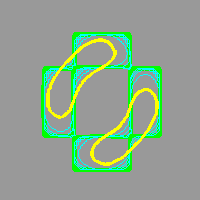
\includegraphics[width=0.22\textwidth]{images/demo/curvature_flow/curvature_flow5}	&
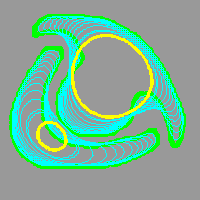
\includegraphics[width=0.22\textwidth]{images/demo/curvature_flow/curvature_flow6}	&
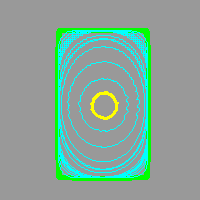
\includegraphics[width=0.22\textwidth]{images/demo/curvature_flow/curvature_flow7}	&
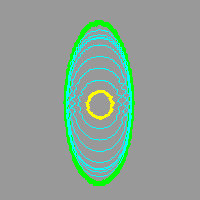
\includegraphics[width=0.22\textwidth]{images/demo/curvature_flow/curvature_flow8}
\end{tabular}
\caption[Motion by mean curvature.]{Example of motion by mean curvature. Initial curve is shown in green and the result after 500 iterations is shown in yellow. Intermediate stages of curve evolution are shown in cyan.}
\label{fig:mean_curvature_demo}
\end{figure}
For 3D applications, we have a closed surface instead of a curve. An area minimizing regularizer can be obtained by replacing the curvature term $\kappa$ in 2D by $H$ which is the sum of the principal curvatures of the surface in 3D \cite{caselles_minimal_surface}. However, unlike the 2D case, mean curvature motion is not the optimal area minimizing flow and there has been other models proposed in the literature \cite{caselles_minimal_surface,tannenbaum1997invariant}.

\subsection{Malladi-Sethian model}
The  above mentioned motion models are not really suitable for object segmentation, since neither (\ref{eq:const_speed}) or (\ref{eq:curvature_motion}) consider any information from the image. Malladi and Sethian \cite{malladi_sethian} introduced a flow based on the image model for object segmentation based on the gradient of the image. If $g(|\nabla f|)$ is a function which assumes a high value at the homogeneous portions of the image and significantly low value($\approx 0$) at the edges. One particular realization may be computed as $g=1/(1+|\nabla f|^q)$. With this definition, the curve motion equation is realized as:
\bea
\textbf{C}_t = g(|\nabla f|)(c_0+\kappa)\;\textbf{n}
\label{eq:malladi_sethian}
\eea
The function $g(.)$ acts as an edge indicator, by slowing down the speed of the snake when it approaches an edge, characterized by high gradient value. As before, the sign of the scalar $c_0$ dictates whether the snake moves outward or inward. The curvature based term imparts smoothness to the solution by disallowing irregular contour shapes.


\subsection{Geodesic Active Contour (GAC)}
Caselles et al.\cite{caselles_GAC} realized a drawback of Malladi's model which restricted its applicability in certain scenarios. This is because the function $g(.)$ does not stop the snake propagation at the edges, but merely slows it down. Therefore, if the edge strength is not significant enough, the propagating curve may not converge at the boundary but continue its motion and eventually collapse or diverge out.
\bea
\textbf{C}_t = g(|\nabla f|)(c_0+\kappa)\;\textbf{n}-\langle\nabla g,\textbf{n} \rangle \;\textbf{n}
\label{eq:GAC}
\eea
\begin{figure}[t]
\centering
\renewcommand{\tabcolsep}{0.05cm}
\begin{tabular}{@{}ccc@{}}

\includegraphics[width=0.3\textwidth]{images/demo/GAC/blobs_gaussian}	&
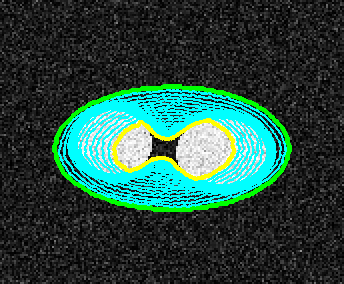
\includegraphics[width=0.3\textwidth]{images/demo/GAC/malladi_bad}	&
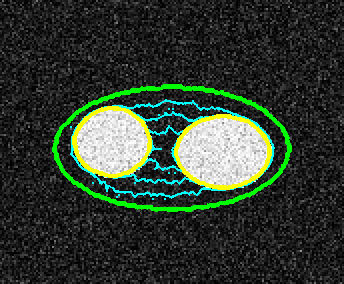
\includegraphics[width=0.3\textwidth]{images/demo/GAC/GAC_good}	\\
(a) original image & (b) Malladi-Sethian  & (c) GAC
\end{tabular}
\caption[GAC vs Malladi-Sethian model]{Segmentation performance of geodesic active contour model over Malladi-Sethian's method. The initial curve is shown in green and the final contour in yellow. Intermediate steps are shown in cyan.}
\label{fig:GACvsMalladi}
\end{figure}

The first part of (\ref{eq:GAC}) is similar to that of Malladi's model. The second term improves the evolution by incorporating a speed term which attracts the evolving curve towards the edge. This results in an additional component which halts the snake at the object boundaries. This is particularly helpful, since the function $g(.)$ does not stop the curve from leaking across the edges; it merely slows down the propagation speed. With the additional attraction term, the moving contour is attracted toward the edges and forces the curve to stop moving (see Fig.~\ref{fig:GACvsMalladi}).

 
This model can be interpreted as a flow that minimizes the geodesic curve length instead of the euclidean length, which makes it a geodesic length minimizing flow. For further detail, we refer the reader to the original paper\cite{caselles_GAC}.

\section{Implementation using level sets}
The previous subsection describes a few important active contour models. With a model already developed, the next challenge is that of implementation. This is where two subtypes of active contours emerge: \textit{parametric} and \textit{geometric}.

One way to implement the curve evolution equation (\ref{eq:curve_evolve_general}) is via discrete parametrization of the curve. The curve is represented by a set of finite number of contour pixels (or \textit{snaxels}), and the curve evolution is computed by explicitly calculating the deformation forces at these contour positions. Such algorithms fall under the category of parametric active contours and there has been significant research in this domain, involving both theoretical aspects
\cite{kwt_snakes,li_VFC,xu_GVF_journal,li_PIG,jacob2004efficient,bspline_snake,mishra2011decoupled} and practical applications\cite{leucocyte_dipti,ray2003merging,ray2002tracking,lesage2009review,zhu2014complete}. 

Parametric active contour methods are generally topology preserving, i.e., the topology of the evolving contour remains same during the motion. While this property may be desired in certain applications (e.g. tracking rigid objects), certain applications demand a methodology which is topology adaptive. For example, when multiple objects are present, one may wish to design an active contour model, which is capable of detecting each object despite starting from a single initialization. Unfortunately, parametric methods are incapable of handling changes in topology, unless specialized algorithms are developed to perform contour merging or splitting.

\subsection{Geometric active contour}
Osher and Sethian\cite{osher_sethian} proposed an implicit curve evolution method which makes the curve adaptive to the topology of the objects. This set of algorithms, popularly known as level set methods or geometric active contour methods represent the contour $\textbf{C}(\textbf{x},t)$  as the zero level set of a continuous functional $\phi$. With this representation, the curve evolution is obtained explicitly, by  deforming the functional $\phi$ instead of calculating the forces on the discretized contour positions. The function $\phi:\Omega\times\mathbb{R}^+\mapsto\mathbb{R}$ is defined such that the active contour is given by $\textbf{C}(\textbf{x},t)=\lbrace\textbf{x}:\phi(\textbf{x},t)=0\rbrace\;\forall t\in\mathbb{R}^+$. Furthermore, if $\Gamma_{in}\subseteq\Omega$ and $\Gamma_{out}\subseteq\Omega$ denote the regions inside and outside the zero level set of $\phi$, we have $\phi(\textbf{x}) \geq 0\; \forall \textbf{x}\in\Gamma_{in}$ and  $\phi(\textbf{x}) < 0\; \forall \textbf{x}\in\Gamma_{out}$.

The advantage of using the embedding functional $\phi$ is that all operations are carried out on $\phi$ and the evolving contour is represented by the zero level set of $\phi$. Using this implicit representation of the curve enjoys the benefit of topological adaptivity; the embedding function has natural ability of merging and splitting -- which subsequently allows the zero level set to merge and split without the use of specialized schemes. 

Naturally, the next question is how to modify (\ref{eq:curve_evolve_general}) so that the implicit motion can be accommodated? As it turns out, it is quite trivial to develop a relationship between the explicit motion model and the implicit model. Assuming that the curve motion equation is given by (\ref{eq:curve_evolve_general}), the explicit motion model is given by
\bea
\phi_t + \langle\textbf{C}_t,\nabla\phi \rangle = 0
\label{eq:explicit_motion_ls}
\eea
The outward normal vector and curvature are computed as
\bea
\textbf{n}&=&-\dfrac{\nabla\phi}{|\nabla\phi|}\\
\kappa&=&\text{div}\left(\dfrac{\nabla\phi}{|\nabla\phi|}\right)
\label{eq:normal_curvature_ls}
\eea
Derivation details are given in the Appendix. Now that we have obtained an equivalence between the implicit and explicit representations, we can modify the curve motion models in the level set framework. 

\begin{table}[bht]
\centering
\caption[Geometric Flow]{Equivalent geometric flow equations using level set representation.}
\begin{tabular}{c|c|c}
Motion model & Curve motion model & Geometric model \\
\hline \hline 
Constant speed motion & $\textbf{C}_t=c_0\, \textbf{n}$ & $\phi_t=c_0|\nabla
\phi|$ \\
Mean curvature motion & $\textbf{C}_t=\kappa\, \textbf{n}$ & $\phi_t=\text{div}\left(\dfrac{\nabla\phi}{|\nabla\phi|}\right)|\nabla
\phi|$ \\
Malladi-Sethian model & $\textbf{C}_t=g(.)\left(c_0+\kappa\right) \textbf{n}$ & $\phi_t=g(.)\left(c_0+\kappa\right)|\nabla
\phi|$ \\
Geodesic active contour & $g(.)\kappa\;\textbf{n}-\langle\nabla g,\|\textbf{n} \rangle \;\textbf{n}$ & $\phi_t= \text{div}\left(g(.)\dfrac{\nabla\phi}{|\nabla\phi|}\right)|\nabla\phi|$\\
\hline
\end{tabular}
\label{table:geometric_flow}
\end{table}
Explicit curve motion equation involving the embedding function is popularly known as \textit{geometric flow} equation. The benefit of the geometric model is its topological flexibility. Such models are very efficient in segmenting multiple objects and have been used for numerous applications in image analysis. Implementation of the geometric flow is performed by discretizing the function $\phi$ over an uniform grid and using tools from numerical methods to solve the partial differential equation. 

It is desirable that the embedding function is a differentiable function which is positive inside the zero level set and negative outside it. Also, since the zero level set of $\phi$ gives the position of the contour at each step of iteration, it is important to maintain the property of $\phi$ during the flow. This is performed by a process known as \textit{reinitialization} which allows $\phi$ to retain the properties of a geometric embedding function and  prevents instability. Several reinitialization techniques have been proposed in the literature including pde based methods and variational methods\cite{osher_sethian,caselles_geodesic,li_without_reinit_CVPR,li_DRLS}. 


While topology adaptability is a feature of geometric models which is unavailable with the parametric setup, one loses out in terms of computational time. While parametric models operate on a set of discrete points, the geometric models demand the entire functional $\phi$ to be updated at each interval. There has been concerted efforts to reduce the computational time of such methods which includes narrow band methods (where update is performed only at positions near the zero level sets), fast marching and multigrid methods\cite{malladi_sethian,papandreou2007multigrid,goldenberg2001fast,sethian1999fast,shi2008real}. 

\section{Variational active contours}

In the previous sections, we have described active contour models in a top down fashion. An equation for propagating the curve is first established and then implicit curve motion is obtained by using an embedding functional. Designing such models generally involve computing a suitable speed function $F$ (see eq. (\ref{eq:curve_evolve_general})). In many cases, it is convenient to design a solution by finding a suitable speed function or force function. This force function typically consists of a smoothness invoking part and an image based component which generally attracts the level set to the regions of high gradient in the image\cite{malladi_sethian,caselles_geodesic}. Consequently, such techniques are categorized as  \textit{edge based} techniques.

However, in certain applications, the object segmentation may be performed as a (possibly local) solution to a suitable optimization problem. A popular example is that of region based segmentation framework proposed by Mumford and Shah \cite{mumford_shah}. The authors introduced a segmentation methodology which attempts to cluster the image into sets of foreground and background pixels based on their gray level intensity.
The variational segmentation methodology can be mathematically stated as follows:
\bea
\phi^*&=&\underset{\phi}{\arg\!\min}\;\mathcal{E}(\phi) \label{eq:variational_ls_basic}
\\
\phi_t &=& -\nabla_{\phi}\;\mathcal{E}(\phi)
\label{eq:variational_grad_flow}
\eea
The zero level sets of the local minimizer $\phi^*$ of an energy functional $\mathcal{E}(\phi)$ corresponds to the detected object boundaries (eq. (\ref{eq:variational_ls_basic})). Generally, a gradient descent based algorithm is deployed to find the local minima of the functional and the solution is computed iteratively. The gradient descent equation (\ref{eq:variational_grad_flow}) corresponds to the curve propagation partial differential equation (similar to (\ref{eq:curve_evolve_general})) for the variational scheme which is derived using variational calculus\cite{calc_of_var}. This equation is often referred to as \textit{variational flow equation} or \textit{gradient flow equation}. 

The variational problem requires specification of the energy functional $\mathcal{E}(\phi)$. Traditionally, an energy function consists of two terms-- a regularization term $\mathcal{E}_r(\phi)$ which generates smooth solution and another data term $\mathcal{E}_d(\phi,f(\textbf{x}))$ which usually incorporates image based features for segmentation \cite{zhao_variational,chan_vese,bernard_splinedCV,lankton_localCV}. In addition, segmentation performance can be significantly improved by incorporating prior information about the object shape . Variational formulations provide an elegant way to introduce such priors in form of an additive energy term and may be introduced both as a hard prior\cite{chan_LS_shape,cremers2007review,foulonneau2006affine,gooya2008variational} or a soft prior\cite{nain2004vessel}.

\subsection{Variational contour regularization}
Here we discuss two popularly used energy functionals used for the purpose of obtaining a smooth active contour. One way to regularize the shape of the contour is by restricting its total length. This is performed by minimizing eq. (\ref{eq:length_reg}), and the gradient flow equation is obtained by deriving the Euler-Lagrange equation and using gradient descent for local solution. This is shown in eq. (\ref{eq:length_reg_flow}).
\bea
\mathcal{E}_{r}^{(1)}&=&\int_{\Omega}|\nabla H(\phi)|d\textbf{x} \label{eq:length_reg} \\
\phi_t&=&\text{div}\left(\dfrac{\nabla \phi}{|\nabla \phi|}\right)\delta\left(\phi\right)
\label{eq:length_reg_flow}
\eea
Here $H(.)$ is the Heaviside function defined such that $H(y)=1\; \forall y>=0$ and $H(y)=0$ otherwise. In otherwise, the Heaviside function serves as an indicator function for the area inside the zero level set of $\phi$. $\delta(.)$ is the Dirac delta function. Since the Heaviside function is not differentiable, for practical purposes the following regularized versions of the Heaviside and Dirac functions are used\cite{chan_vese}. 
\bea
\heav(q)&=& \dfrac{1}{2}\left(1+\dfrac{2}{\pi}\tan^{-1}\left(\dfrac{q}{\epsilon}\right)\right) \label{eq:heav_relax} \\
\dirac(q) &=& \dfrac{d}{dq}\heav(q) \label{eq:dirac_relax}
\eea
Analyzing eq. (\ref{eq:length_reg}), it is not difficult to comprehend that the right hand side of the equation corresponds to the total length of the zero level set of $\phi$. Therefore, eq. (\ref{eq:length_reg_flow}) represents the curve evolution equation such that the length of the curve is locally minimized. One can find a similarity between the length shortening gradient flow (\ref{eq:length_reg_flow}) and the mean curvature motion in (\ref{eq:curvature_motion}), where the expressions differ by the multiplicative terms. In fact, if only a narrow band around the zero level contour is considered, one can find that both these formulations lead to almost identical solutions that regularizes the curve via length minimization.


Another regularization popularly  used for getting a smooth solution is obtained by minimizing the total area inside the contour. The area minimizing smoothing functional and the corresponding gradient flow equation are computed as follows:
\bea
\mathcal{E}_{r}^{(2)}&=&\int_{\Omega}\heav(\phi)d\textbf{x} \label{eq:area_reg} \\
\phi_t&=&-\dirac(\phi) \label{eq:area_reg_flow}
\eea
The regularizing energy functional contributes only to the smoothness of the solution. The regularizers are generally not dependent on image features. however, to perform segmentation, one needs to engineer a suitable data term that incorporates image based information (such as intensity, edge strength, texture etc.) to drive the level sets toward the desired object boundaries.
 
\subsection{Chan-Vese's segmentation model}
Chan and Vese\cite{chan_vese} proposed a level set formulation to minimize the Mumford Shah functional \cite{mumford_shah} for segmentation. The Chan-Vese framework models the image as a set of constant illumination regions and performs a two-class segmentation by computing the optimal partition which satisfies the constant illumination constraint. The authors also propose a multi-phase variant \cite{vese_multiphase} of their approach to perform multi class grouping. 

The piecewise constant model of Chan-Vese\cite{chan_vese}  models the object foreground and background by the scalars $c_1$ and $c_2$. In a level set framework, the Chan-Vese energy functional $\mathcal{E}_d=\mathcal{E}_{CV}$ is written as follows:
\bea
\mathcal{E}_{CV}(\phi,c_1,c_2)= \int_{\Omega}|f(\textbf{x})-c_1|^2H(\phi) d\textbf{x} 
						   +\int_{\Omega}|f(\textbf{x})-c_2|^2 \left(1-H(\phi)\right) d\textbf{x}  
\label{eq:chan_vese}
\eea
Here $f(\textbf{x})$ is the image defined over the domain $\Omega$. The $\phi$ that locally minimizes (\ref{eq:chan_vese}) creates segments in a manner such that the foreground and background are best approximated by the intensity levels $c_1$ and $c_2$.


The (local) minima of (\ref{eq:chan_vese}) is obtained using alternate minimization. In the first step, the optimal values of the scalars $c_1,c_2$ are obtained as follows:
\bea
c_1^*,c_2^*& = &\underset{c_1,c_2}{\arg\!\min}\, \mathcal{E}_d(\phi,c_1,c_2) \\
\phi^* & = & \underset{\phi}{\arg\!\min}\, \mathcal{E}_d(\phi,c_1^*,c_2^*)
\eea
The solution for $c_1^*\,\text{and} c_2^*$ is obtained in closed form as 
\bea
c_1^* = \dfrac{\int f(\textbf{x})\heav(\phi)d\textbf{x}}{\int \heav(\phi)d\textbf{x}},\;
c_2^* = \dfrac{\int f(\textbf{x})\left(1-\heav(\phi)\right)d\textbf{x}}{\int \left(1-\heav(\phi)\right)d\textbf{x}}
\label{eq:cv_scalars}
\eea
With these updated values, the local optima for the embedding function $\phi$ is computed by iteratively solving the following gradient flow equation.
\bea
\phi_t = \left[-(f(\textbf{x})-c_1^*)^2+(f(\textbf{x})-c_2^*)^2\right]\dirac(\phi)
\label{eq:cv_flow}
\eea

In addition to (\ref{eq:cv_flow}), a regularizer term as in (\ref{eq:length_reg_flow}) is also added to obtain smooth boundaries. The above mentioned model is particularly useful when the object edges are not prominent or the edges are blurred.  Also, region based methodologies exhibit significant performance benefits for noisy images where the accuracy of the edge map is sacrificed due to noise. 


\section{Edge based vs. region based models}

\subsection{Synthetic examples}
Fig.~\ref{fig:GACvsCV} compares the performance of Geodesic Active Contour \cite{caselles_geodesic} algorithm which is an edge based framework versus the region based segmentation technique due to Chan and Vese\cite{chan_vese}. To demonstrate the properties of each algorithm, we simulate four images. The first image is that of a disc (Fig.~\ref{fig:GACvsCV}(a), row 1) with homogeneous intensity level. This image has uniform illumination and the edges are well defined. Therefore, such an image is a good candidate for segmentation with either edge based or region based approaches. It is observed that both the algorithms perform almost identically in this case.
\begin{figure}[tb]
\centering
\renewcommand{\tabcolsep}{0.05cm}
\begin{tabular}{@{}ccc@{}}
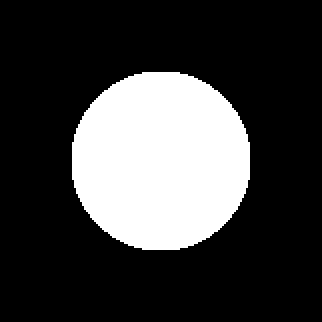
\includegraphics[width=0.3\textwidth]{images/demo/GACvsCV/disk}	&
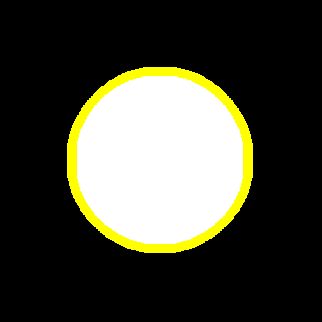
\includegraphics[height=0.3\textwidth]{images/demo/GACvsCV/GAC_disc}	&
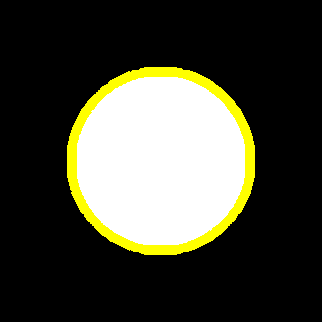
\includegraphics[height=0.3\textwidth]{images/demo/GACvsCV/CV_disc}	\\
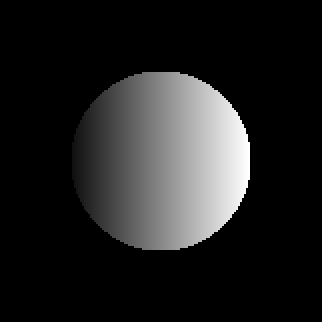
\includegraphics[width=0.3\textwidth]{images/demo/GACvsCV/inhom}	&
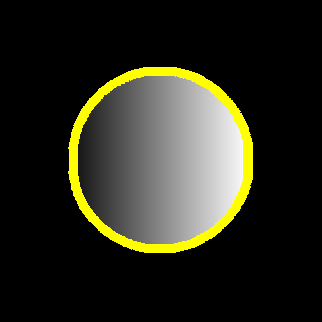
\includegraphics[height=0.3\textwidth]{images/demo/GACvsCV/GAC_inhom}	&
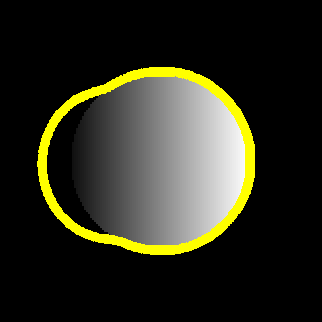
\includegraphics[height=0.3\textwidth]{images/demo/GACvsCV/CV_inhom}	\\
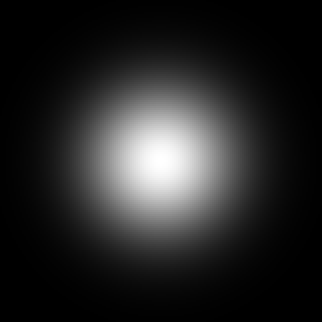
\includegraphics[width=0.3\textwidth]{images/demo/GACvsCV/gauss}	&
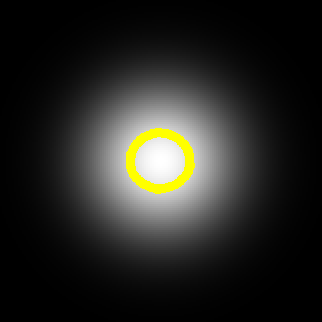
\includegraphics[height=0.3\textwidth]{images/demo/GACvsCV/GAC_gauss}	&
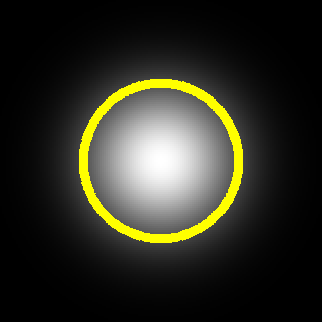
\includegraphics[height=0.3\textwidth]{images/demo/GACvsCV/CV_gauss}	\\
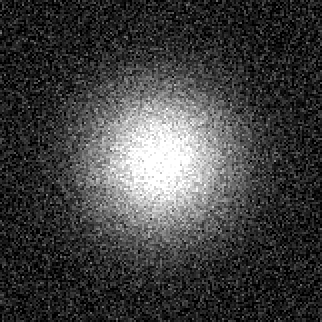
\includegraphics[width=0.3\textwidth]{images/demo/GACvsCV/gauss_noisy}	&
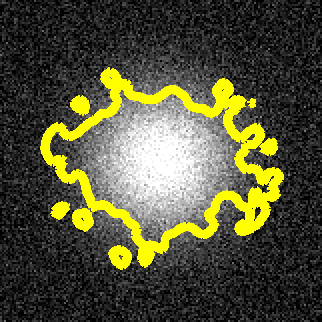
\includegraphics[height=0.3\textwidth]{images/demo/GACvsCV/GAC_gauss_noisy}	&
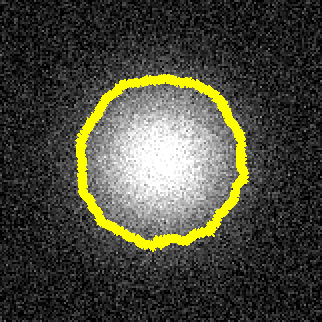
\includegraphics[height=0.3\textwidth]{images/demo/GACvsCV/CV_gauss_noisy}	\\
(a) simulated image & (b) GAC\cite{caselles_GAC} & (c) Chan-Vese\cite{chan_vese}
\end{tabular}
\caption[Edge based model vs region based model]{(a)Simulated images. (b)Segmentation performance of (GAC\cite{caselles_GAC}) and (c) Results via (Chan-Vese\cite{chan_vese}). The final result is shown by the yellow contour.}
\label{fig:GACvsCV}
\end{figure}

The second image (Fig.~\ref{fig:GACvsCV}(a), row 2) is that of a disc with non uniform intensity. However, the object edges are still relatively well defined. As a result, almost perfect segmentation is obtained using the GAC model. However, Chan and Vese's algorithm is incapable of handling intensity inhomogeneity. This is a significant deficiency of this method and it would be dealt with substantial rigor in the next chapter. The piecewise constant illumination model of Chan-Vese fails to produce correct segmentation, and we observe false positive in (Fig.~\ref{fig:GACvsCV}(c), row 2).

In the third example (Fig.~\ref{fig:GACvsCV}(a), row 3), the edges of the disc are blurred by smoothing it with a Gaussian filter. As expected, the edge based algorithm fails to identify the proper object boundary, whereas the region based technique performs significantly better.

Finally, the fourth image (Fig.~\ref{fig:GACvsCV}(a), row 4) is simulated by adding zero mean Gaussian noise to the blurry disc image. We observe that region based segmentation is particularly robust against additive noise and the segmentation performance is not degraded significantly. On the other hand, GAC model faces difficulties both due to blurred edges as well as signal noise.

\subsection{Real examples}
\begin{figure}[t]
\centering
\renewcommand{\tabcolsep}{0.05cm}
\begin{tabular}{@{}ccc@{}}
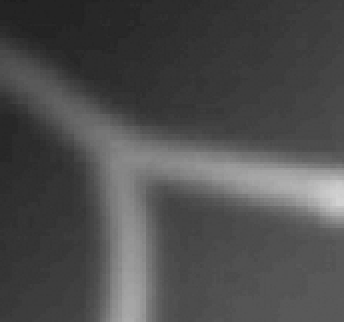
\includegraphics[width=0.3\textwidth]{images/L2S_compare/orig_1}	&
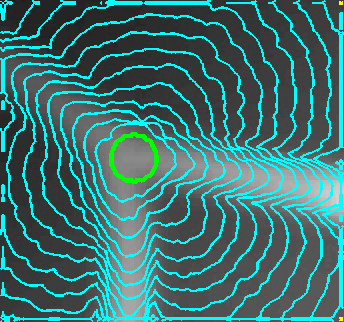
\includegraphics[width=0.3\textwidth]{images/L2S_compare/GAC_1}	&
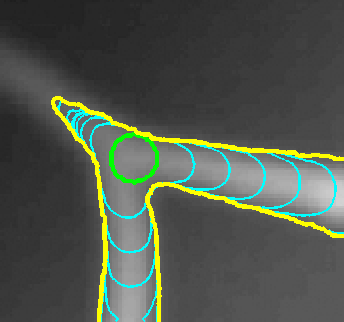
\includegraphics[width=0.3\textwidth]{images/L2S_compare/CV_1}	\\
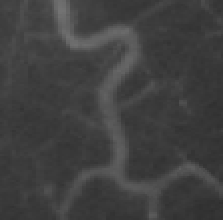
\includegraphics[width=0.3\textwidth]{images/L2S_compare/orig_4}	&
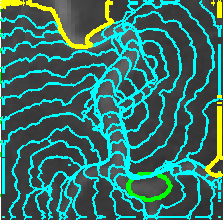
\includegraphics[width=0.3\textwidth]{images/L2S_compare/GAC_4}	&
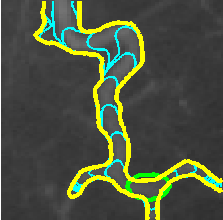
\includegraphics[width=0.3\textwidth]{images/L2S_compare/CV_4}	\\
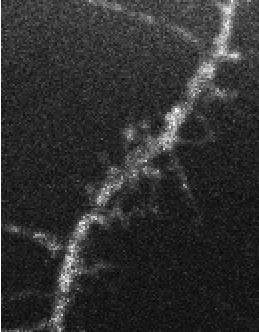
\includegraphics[width=0.3\textwidth]{images/L2S_compare/orig_5}	&
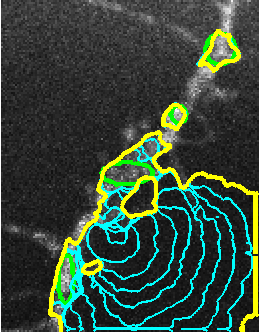
\includegraphics[width=0.3\textwidth]{images/L2S_compare/GAC_5}	&
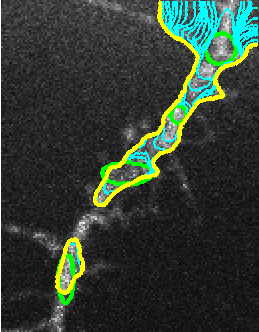
\includegraphics[width=0.3\textwidth]{images/L2S_compare/CV_5}	\\
(a) original image & (b) GAC & (c) Chan Vese
\end{tabular}
\caption[Geometric Snakes: negative examples]{Cases of improper segmentation using geometric contours. (a) Five images including simulated and real examples with varying illumination and weak edges. (b) Shows segmentation using geodesic active contour and (c) Shows segmentation due to Chan-Vese's method. The initial contour is plotted in green and the final contour in yellow. Intermediate steps of curve evolution are shown in cyan. This figure is best viewed in color.}
\label{fig:ls_compare}
\end{figure}
In Fig.~\ref{fig:ls_compare}, comparitive study of segmentation performance of geodesic active contour model and Chan-Vese's technique is presented on a set of real images consisting of vascular structures (neurons and retinal blood vessels) imaged using fluorescence microscope. Fluorescence microscopy images are often plagued by noise, inhomogeneous intensity and low contrast which leads to poor edge strength. 
As a result, we find that neither \cite{caselles_geodesic} nor \cite{chan_vese} is perfectly suitable for segmentation under such conditions. Segmentation error is caused either due to the curve leakage phenomenon (Fig.~\ref{fig:ls_compare}(b)) or under segmentation (Fig.~\ref{fig:ls_compare}(c)). In the following chapter, we attempt to design a generic segmentation algorithm which is tolerant to the commonly occurring artifacts in fluorescence microscopy.

\section{Discussion} 
In this chapter we have provided a broad overview of geometric active contours. Geometric contours are topology adaptive which makes them particularly attractive choice for segmentation. The segmentation model is either described in terms of explicit curve motion equation (\ref{eq:curve_evolve_n&t}) and then implemented by implicit representation of the contour as the zero level curve of an embedding functional (\ref{eq:explicit_motion_ls}). Another popular way to describe the segmentation process is via variational formulation which involves minimization of a suitable energy functional using variational calculus. The gradient flow equation (\ref{eq:variational_grad_flow}) is derived using gradient descent technique for computing the local minima of the functional. In either case, segmentation is performed by iteratively propagating the zero level set of the embedding function on a discrete grid borrowing tools from numerical mathematics.

Both formulations are widely used in the community and they enjoy their own sets of benefits. While curvature flow equations are often easy to conceptualize (e.g. equavalent to physical curve motion models such as wave propagation), variational models have gained popularity because of the flexibility to add further constraints in the solution in terms of shape prior. We also showed that in many cases it is possible to draw an analogy between the curve flow equations derived from the two techniques and in a majority of cases the results are quite comparable.

We then presented a comparison between edge based and region based methods for segmentation. It is shown that edge based models are more suitable for clean signals with strong edge response. Furthermore, such models are less susceptible to error if the object gray value is non homogeneous. Region based methods, on the other hand, are more robust to noise and do not depend particularly on the edge strength of the signal. However, it was demonstrated that the performance can degrade significantly in presence of intensity inhomogeneity. 

In the next chapter we focus our attention on segmenting vascular structures from 2D fluorescence microscopy images. As we have discussed briefly, fluorescence microscopy imagery are charecterized by poor contrast and varyinng intensity levels of the object.  This restricts the performance of the popular traditional geometric active contour models. This motivates us to develop a geometric segmentation model which is capable of handling noise and contrast fluctuations in the images.


%% Chapter 3
\setstretch{1} 
\chapter{2D segmentation with level sets} % Main chapter title
\setstretch{2} 
\label{Chapter3} % For referencing the chapter elsewhere, use \ref{Chapter2} 

\lhead{Chapter 4. \emph{L2S and DL2S}} % This is for the header on each page - perhaps a shortened title

%----------------------------------------------------------------------------------------
In the previous chapter we discussed potential benefits of using geometric active contours or snakes for certain segmentation problems. Geometric snakes are capable of adapting to the topology of the objects and  their ability to elastically deform and delineate object boundaries with sub-pixel accuracy make these methods attractive choice for several biomedical image analysis applications. 

We have also elaborated how region based models are more suitable for segmenting images with weak edges and noisy structures. One of the more popular region based algorithm was proposed by Chan and Vese\cite{chan_vese} where they model the image as a set of flat zones or regions with constant gray value. The authors also propose a multi-phase variant \cite{vese_multiphase} of their approach to perform multi-class grouping. 

The constant illumination assumption is challenged in applications where the signal intensity is inhomogeneous. This is encountered frequently in many medical and biological imaging applications like magnetic resonance (MR) imaging, ultrasound, X-ray, confocal and electron microscopy, etc. While edge based techniques are better suited for non uniformly illuminated images, low SNR and weak edges of biological structures limit their general applicability.

\section{Application to 2D neuron image tracing}

Before dealing with the 3D confocal images, which require more sophisticated processing, we first propose a segmentation algorithm which would work on relatively simpler 2D images. A 2D image is obtained from its 3D counterpart by taking a mean intensity projection along its vertical axis. While we want to eventually develop a 3D tracer, we hypothesize that analyzing 2D neuron images serves as a strong platform for designing our 3D tracer. It is evident that some structural information of the neurons are lost when the image dimension is reduced by projecting it to a 2D space. However, there are several interesting issues which demand our attention even after this simplification. First, even after conversion  2D, we still retain substantial information about a neuron's morphology and this is why there exists a number of popular tracers which have been developed specifically for 2D processing \cite{basu2010tree2tree,meijering2004design}. Second, with the reduced dimension, one may perform computation at a much faster rate than in 3D, thereby making 2D analysis an attractive choice for an initial, global assessment of the neurites. Finally, the 2D conversion introduces further challenges for image processing, including introduction of intensity inhomogeneity, which occurs due to signal attenuation by the tissues at greater depths. It is a challenge in itself to investigate the applicability of state of the art segmentation algorithms on these datasets and understand the special processing needs for further robust analysis.

\section{Background and motivation}
In this chapter we introduce an edge oblivious segmentation approach \emph{Legendre Level Set} (L2S), which is robust to smooth variations in region intensity levels. State of the art techniques that tackle inhomogeneity typically require some form of local processing. However, while a global method like Chan-Vese's is insufficient in handling large scale intensity variations, a strictly local approach may lead to undesired segmentation artifacts, especially in presence of noise. We aim to eradicate these issues by proposing a generalized solution for region based segmentation in presence of significant intensity variation and additive noise. 

Chan and Vese's region based technique is mathematically summarized in (\ref{eq:chan_vese}). The locally optimum level set embedding function $\phi^*$ that minimizes (\ref{eq:chan_vese}) partitions the image in two regions such that the foreground and background are best approximated by the scalars $c_1$ and $c_2$, which are computed using alternate minimization.

As mentioned previously, this model is incapable of handling spatially varying illumination. A solution was proposed in \cite{vese_multiphase}, where the authors replaced the scalars $c_1,c_2$  with smooth functions $c_1(\textbf{x})$ and $c_2(\textbf{x})$ in (\ref{eq:chan_vese_PS}).
\bea
\mathcal{E}_{CV}(\phi,c_1(\textbf{x}),c_2(\textbf{x}))&= \displaystyle\int_{\Omega}|f(\textbf{x})-c_1(\textbf{x})|^2\heav(\phi) d\textbf{x} + \int_{\Omega}|f(\textbf{x})-c_2(\textbf{x})|^2\heav(\phi) d\textbf{x} \nn
\\&+\displaystyle s_1\int_{\Omega}|\nabla c_1(\textbf{x})|d\textbf{x} + s_2\int_{\Omega}|\nabla c_2(\textbf{x})|d\textbf{x}
\label{eq:chan_vese_PS}
\eea
Smoothness of the functions are established by regulating their total variation, controlled by the parameters $s_1,s_2$. As before, alternating minimization is used to solve (\ref{eq:chan_vese_PS}). However, unlike (\ref{eq:chan_vese}), the polynomials are computed numerically as shown below, by deriving the EL equations and using gradient descent for local minimization.
\bea
\dfrac{\partial c_1(\textbf{x})}{\partial t} &=& 2(f(\textbf{x})-c_1(\textbf{x}))\heav
(\phi) + s_1 \text{div}\left(\dfrac{\nabla c_1(\textbf{x})}{|\nabla c_1(\textbf{x})|}\right) \nn \\
\dfrac{\partial c_2(\textbf{x})}{\partial t} &=& 2(f(\textbf{x})-c_2(\textbf{x}))\heav(\phi) + s_2 \text{div}\left(\dfrac{\nabla c_2(\textbf{x})}{|\nabla c_2(\textbf{x})|}\right) \nn \\
\dfrac{\partial \phi}{\partial t} &=& \left[-(f(\textbf{x})-c_1^*(\textbf{x}))^2+(f(\textbf{x})-c_2^*(\textbf{x}))^2\right]\dirac(\phi)
\label{eq:PS_solution}
\eea
While the solution is attractive, this piecewise smooth model is computationally expensive. This is because, in order to calculate the locally optimum level set function $\phi^*$, one needs to iteratively calculate the optimum polynomials $c_1^*(\textbf{x})$ and $c_2^*(\textbf{x})$ by numerically solving (\ref{eq:PS_solution}) thereby making computation significantly expensive. 

Recently, Li \textit{et al}. \cite{li_region_scalable} introduced a region scalable model to localize the energy functional. The region localization is controlled by the scale of a Gaussian kernel, which is manually tuned for optimal performance. Efforts have been made to incorporate the region statistics for segmentation \cite{kim_nonparametric,cremers2007review}. These methods are robust to initialization and relatively less sensitive to noise. However, Lankton \textit{et al}.\cite{lankton_localCV} demonstrated that global statistics may not be the best resort for segmenting inhomogeneous objects. Instead, the authors generalize the local region based methods, by proposing a generic energy functional capable of performing segmentation using different region based criteria. 
They also show that by judiciously tuning the region localizing mask size, one can achieve high quality segmentation, even in presence of noise and inhomogeneity. 
However, one downside of their approach is that it requires additional local computation, thus increasing the risk of being stuck within local minima. 


Feng \textit{et al}.  \cite{feng2000tomographic} proposed a method for tomographic reconstruction by using a low order parametric model to represent object texture. However, the algorithm is tailored for tomographic reconstruction and is difficult to generalize. Recently a method was proposed to model the foreground and background by a linear function \cite{du_linear_approx}. This approach is an improvement over the model of Chan-Vese, but does not accommodate nonlinear illumination change.  

From the above discussion we observe that a majority of these approaches rely on local information only. While localizing the segmentation energy is essential in dealing with inhomegeneity, a generic global framework is also necessary to avoid the local minima problem. We propose to model the foreground and background illumination by a set of Legendre basis functions \cite{mukherjee_L2S}. This model allows the region intensities to be represented in a lower dimensional subspace, thereby permitting smooth approximation. Low dimensional signal representation has been used in a slightly different context in the literature, primarily to accomodate shape priors for segmentation \cite{fritscher20073d,huang2008metamorphs}.  However, although shape based information assists segmentation, such techniques require an atlas of pre-registered objects, which may be unavailable for general purpose segmentation. 
We further show that the proposed model \textit{Legendre Level Set}(or L2S) is computationally simple, since we achieve a stable, closed form solution at each iteration, which allows faster processing.

\section{2D segmentation using L2S}

The traditional Chan-Vese functional (\ref{eq:chan_vese}) can be reformulated and generalized by replacing the scalars $c_1$ and $c_2$ by   smooth functions $c_1^m(\textbf{x})$ and $c_2^m(\textbf{x})$. These functions are used to model the intensity in the two regions separated by the zero level set curves of $\phi$. The energy functional corresponding to the L2S data term is expressed as follows:
\bea
\mathcal{E}_{L2S}= \int_{\Omega}|f(\textbf{x})-c_1^m(\textbf{x})|^2H(\phi) d\textbf{x} 
						   +\int_{\Omega}|f(\textbf{x})-c_2^m(\textbf{x})|^2 \left(1-H(\phi)\right) d\textbf{x}  
\label{eq:L2S_data}
\eea
The essence of our approach is embedded in computing these functions. By allowing the regions to be modeled by flexible (but smooth) functions, we introduce the local information required to tackle the heterogeneous illumination. This is a notable feature of our algorithm. Unlike (\ref{eq:chan_vese_PS}), where smoothness is obtained by minimizing the total variation term, we only allow inherently smooth polynomials to approximate the region intensities. As we will show in the next few sections, this formulation allows a suitable framework to model the heterogeneity, without significantly sacrificing on computational time.

To preserve the smoothness and flexibility of the functions, we represent them as a linear combination of a few Legendre basis functions as shown below:
\bea
 c_1^m(\textbf{x}) &=& \sum_{k=0}^m\alpha_k\mathcal{P}_k(\textbf{x}) \\ c_2^m(\textbf{x}) &=& \sum_{k=0}^m\beta_k\mathcal{P}_k(\textbf{x})
 \label{eq:l2s_poly}
\eea
 
Here $\mathcal{P}_k$ is a multidimensional Legendre polynomial, which can be written as the outer product of the one dimensional counterparts. The 2-D polynomial is computed as $\mathcal{P}_k(x,y)=p_k(x)p_k(y)$, $\textbf{x}=(x,y)\in \Omega \subset [-1,1]^2$. $p_k$ is a one dimensional Legendre polynomial of degree $k$ defined as
\bea
p_k(x)=	\frac{1}{2^k}\sum_{i=0}^{k}\binom{k}{i}(x-1)^{k-i}(x+1)^i  
\label{eq:legendre}
\eea
The highest degree of the 1D bases is denoted by $m$. Hence, for the 2D case, we would represent the regions by a linear combination of a set of $(m+1)^2$ 2D Legendre basis functions.

\subsection{Optimization of the energy functional}
\begin{figure}[ht]
\centering
\captionsetup{justification=centering}
\renewcommand{\tabcolsep}{0.05cm}
\begin{tabular}{@{}ccc @{}}
	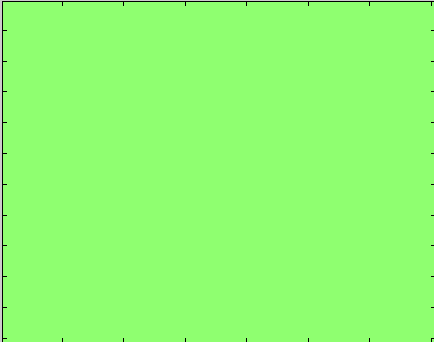
\includegraphics[width=.3\textwidth]{./images/Bases_color/1}  &
	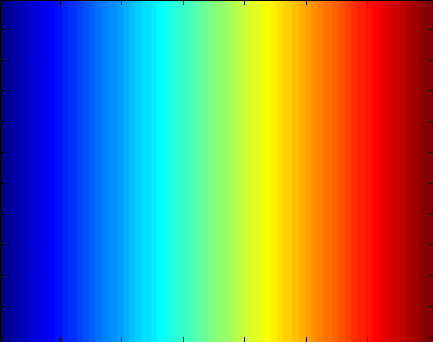
\includegraphics[width=.3\textwidth]{./images/Bases_color/2}  &
	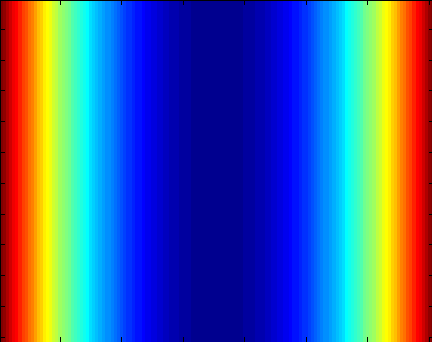
\includegraphics[width=.3\textwidth]{./images/Bases_color/3}  \\
	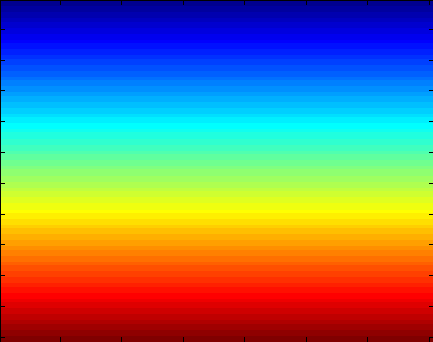
\includegraphics[width=.3\textwidth]{./images/Bases_color/4}  &
	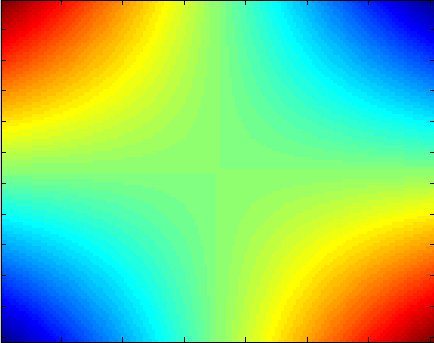
\includegraphics[width=.3\textwidth]{./images/Bases_color/5}  &
	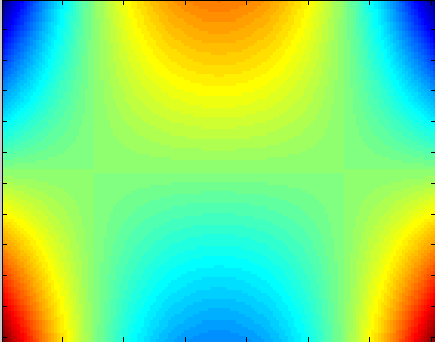
\includegraphics[width=.3\textwidth]{./images/Bases_color/6}  \\
	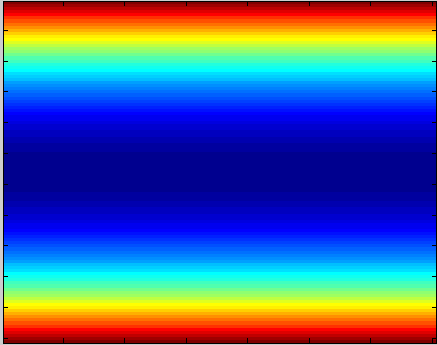
\includegraphics[width=.3\textwidth]{./images/Bases_color/7}  &
	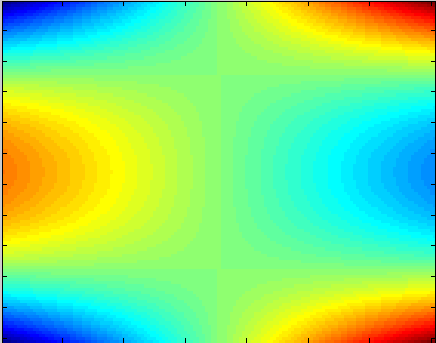
\includegraphics[width=.3\textwidth]{./images/Bases_color/8}  &
	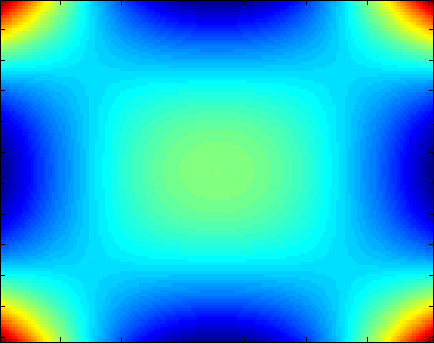
\includegraphics[width=.3\textwidth]{./images/Bases_color/9} 
\end{tabular}
\caption[2D Legendre polynomials]{The set of nine 2D Legendre basis functions. The 2D polynomials are computed from 1D functions of degree 2.}
\label{fig:legendre_bases}
\end{figure}

Let us denote $\mathbb{P}(\textbf{x})=\left(\mathcal{P}_0(\textbf{x}),\ldots, \mathcal{P}_{N}(\textbf{x})\right)^T$ as the vector of Legendre polynomials. $A=\left(\alpha_0,\ldots,\alpha_{N} \right)^T$ and $B=\left(\beta_0,\ldots,\beta_{N} \right)^T$ are the coefficient vectors for the two regions. $N=(m+1)^2$ is the total number of basis functions. We can now rewrite the modified version of (\ref{eq:chan_vese}) in matrix form as
\bea
\mathcal{E}(\phi,A,B)&= \displaystyle\int_{\Omega}\left[|f(\textbf{x})-A^T\mathbb{P}(\textbf{x})|^2 m_1(\textbf{x})+|f(\textbf{x})-B^T\mathbb{P}(\textbf{x})|^2m_2(\textbf{x}) \right]d\textbf{x} \nn \\
						    &+\lambda_1 ||A||_2^2  +\lambda_2 ||B||_2^2 + \nu\, \lint_{\Omega} |\nabla\heav(\phi)| d\textbf{x} 
\label{eq:leg_cv_mat}						  
\eea

In (\ref{eq:leg_cv_mat}) the last term introduces smoothness in the zero level curve, which is regulated by the parameter $\nu$.  Let us also denote  $m_1(\textbf{x})=\heav(\phi)$ and  $m_2(\textbf{x})=1-m_1(\textbf{x})$. 


The non negative regularizing parameters $\lambda_1,\lambda_2$ can be selected using cross validation techniques to avoid over-fitting.
The energy functional (\ref{eq:leg_cv_mat}) is optimized using alternating minimization. In the first step, to find optimal $A$ and $B$, we take the partial derivative of (\ref{eq:leg_cv_mat}) with respect to $A$ and $B$ respectively and setting the result to zero. A closed form solution $\hat{A}$ and $\hat{B}$ is obtained as
\bea
\dfrac{\partial\mathcal{E}(\phi,A,B)}{\partial A}=0 \implies \hat{A} =& \left[K+ \lambda_1 \mathbb{I}\right]^{-1}P \\
\dfrac{\partial\mathcal{E}(\phi,A,B)}{\partial B}=0 \implies \hat{B} =& \left[L+ \lambda_2 \mathbb{I}\right]^{-1}Q 
\label{coef_sol}
\eea
$\left[. \right]$ denotes a matrix. The $N\times 1$ vectors  $P$ and $Q$ are obtained as 
\bea
P=\lint_{\Omega} \mathbb{P}(\textbf{x})f(\textbf{x})m_1(\textbf{x})d\textbf{x} \label{eq:l2s_P}
\\
Q =\lint_{\Omega} \mathbb{P}(\textbf{x})f(\textbf{x})m_2(\textbf{x})d\textbf{x}
\label{eq:l2s_Q}
\eea
Here $\left[K \right]$ and $\left[L \right]$ are Gramian matrices \cite{gramian} of dimension $N\times N$, whose $(i,j)^{th}$ entry are obtained as follows:
\bea
\left[K\right]_{i,j}=& \left<\sqrt{m_1(\textbf{x})}\mathcal{P}_i(\textbf{x}),\sqrt{m_1(\textbf{x})}\mathcal{P}_j(\textbf{x})\right> \\
\left[L\right]_{i,j}=& \left<\sqrt{m_2(\textbf{x})}\mathcal{P}_i(\textbf{x}),\sqrt{m_2(\textbf{x})}\mathcal{P}_j(\textbf{x})\right>
\eea
Here $\left<,\right>$ denotes the inner product operator and $0\leq i,j \leq N$. With the updated coefficient vectors, we can now locally minimize (\ref{eq:leg_cv_mat}) with respect to $\phi$ borrowing techniques from variational calculus. 
The curve evolution is performed by numerically solving the following partial differential equation:
\bea
\frac{\partial \phi}{\partial t}=& \left[-|f(\textbf{x})-\hat{A}^T\mathbb{P}(\textbf{x})|^2 
						   +|f(\textbf{x})-\hat{B}^T\mathbb{P}(\textbf{x})|^2  + \nu \,\text{div}\left(\dfrac{\nabla\phi}{|\nabla\phi|}\right) \right]\dirac(\phi)\nn\\
\label{eq:l2s_gradient_flow}
\eea
We solve (\ref{eq:l2s_gradient_flow}) using gradient descent and initializing $\phi|_{t=0}=\phi_0$ and $\dfrac{\dirac(\phi)}{|\nabla \phi|}\dfrac{\partial\phi}{\partial \hat{n}}=0$ at the domain boundary.

\subsection{Analysis of L2S}
The surface approximate for foreground and background are obtained by computing $\hat{A}^T\mathbb{P}(\textbf{x})$ and $\hat{B}^T\mathbb{P}(\textbf{x})$. Since the coefficient vectors are available in closed form, it makes our algorithm fast and effective. The amount of intensity variation is governed by the coefficient vectors which are computed automatically. However, computing the coefficient vectors require a matrix inversion step. Here we show that the matrices $\left[K\right]$ and $\left[L\right]$ are invertible when the heaviside function is suitably regularized.

Since $\left[K\right]$ is a Gramian matrix, it is full rank iff the polynomials $\sqrt{m_1(\textbf{x})}\mathcal{P}_i(\textbf{x})$, $(i=1,\ldots,N)$ are linearly independent \cite{gramian}. Since the polynomials $\mathcal{P}_i(\textbf{x})$ are linearly independent themselves, it is easy to show that the linear independence holds if $0< m_1(x)< 1$. A similar argument holds for analyzing the invertibility of $\left[L\right]$. 

In \cite{chan_vese}, the authors propose a regularized version of the heaviside function which is given by (\ref{eq:heav_relax})
By this definition, the functions $m_1(\textbf{x})$ and $m_2(\textbf{x})$ are bounded in $\left[0,1\right]$, which make the matrices invertible. 

However, inverting the above mentioned matrices may still be prone to numerical error  when $\sqrt{m_i(\textbf{x})}$ is small. The regularizing constants $\lambda_1$ and $\lambda_2$ contribute to make these matrices well conditioned. Furthermore, the regularization terms are necessary to avoid over-fitting. In most situations, we find that only a few (typically 16) 2-D Legendre functions are sufficient to model the region intensity. However, image noise may lead to over-fitting of the polynomials to the image segments, which may disrupt segmentation as the propagating level set may settle at a local minima. The scalars $\lambda_1,\lambda_2$ produce a damping effect by constraining the $\mathbb{L}_2$ norm of the bases coefficients, thereby favoring interior regions approximated by smooth functions. 

\subsection{Parameter selection for L2S}
Our algorithm requires specification of a few parameters, namely the Legendre polynomial degree $m$ and the regularizing constants $\lambda_1$ and $\lambda_2$ in (\ref{eq:leg_cv_mat}). We experimentally verified that the intensity variation in the images can be adequately modeled by using 1-D Legendre polynomials of (highest) degree three. We found that the algorithm is relatively robust to the selection of this value, but a higher degree polynomial typically requires inversion of a larger matrix, which makes computation significantly more expensive. To estimate the value of $\lambda_1$ and $\lambda_2$, we perform a \textit{leave one out} cross validation on each of the four categories in our dataset. The cross validation is performed over the values of $\{0,1,\ldots,100\}$ in multiples of 2. For simplicity, we have chosen $\lambda_1=\lambda_2$ for every experiment. The particular value which yields the highest average Dice coefficient for each dataset is chosen for experimentation. 


Automated selection of the contour smoothness parameter $\nu$ in (\ref{eq:leg_cv_mat}) is non-trivial. Typically, $0<\nu<1$, where a higher value produces smoother contour. As a rule of thumb, one may wish to set $\nu$ to a relatively higher value if the noise level in the image is high. For our experiments, we observe that the set of ultrasound images and the simulated noisy images require larger values of $\nu$. For all these images, we select $\nu=0.6$. For the less noisy images, $\nu$ is typically set in the range 0.05 to 0.2. 
 
\subsection{Comparison with GAC and Chan-Vese}
\begin{figure*}[th]
\centering
\renewcommand{\tabcolsep}{0.05cm}
\begin{tabular}{@{}cccc@{}}

\includegraphics[width=0.24\textwidth]{images/L2S_compare/orig_2}	&
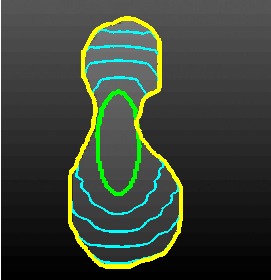
\includegraphics[width=0.24\textwidth]{images/L2S_compare/GAC_2}	&
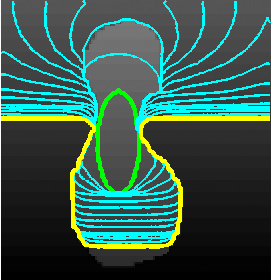
\includegraphics[width=0.24\textwidth]{images/L2S_compare/CV_2}		&
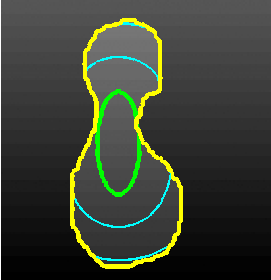
\includegraphics[width=0.24\textwidth]{images/L2S_compare/L2S_2}	
\\
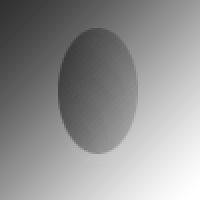
\includegraphics[width=0.24\textwidth]{images/L2S_compare/orig_3}	&
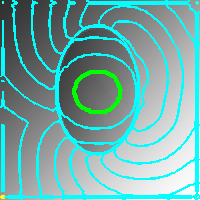
\includegraphics[width=0.24\textwidth]{images/L2S_compare/GAC_3}	&
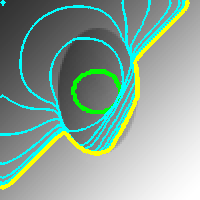
\includegraphics[width=0.24\textwidth]{images/L2S_compare/CV_3}		&
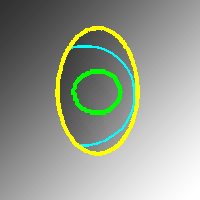
\includegraphics[width=0.24\textwidth]{images/L2S_compare/L2S_3}	
\\
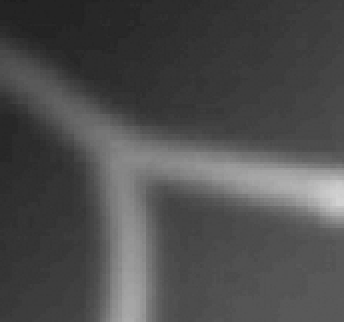
\includegraphics[width=0.24\textwidth]{images/L2S_compare/orig_1}	&
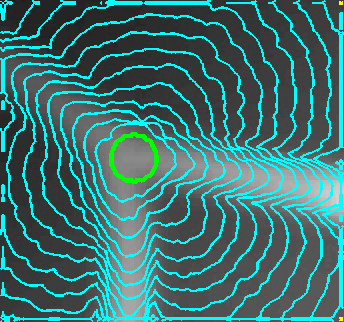
\includegraphics[width=0.24\textwidth]{images/L2S_compare/GAC_1}	&
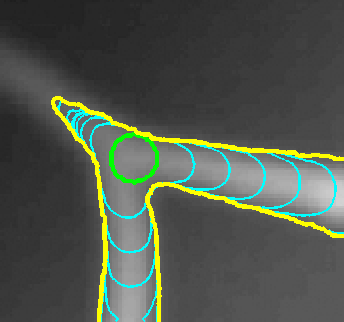
\includegraphics[width=0.24\textwidth]{images/L2S_compare/CV_1}		&
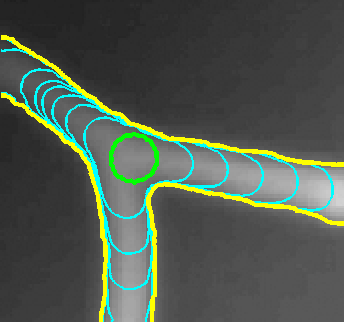
\includegraphics[width=0.24\textwidth]{images/L2S_compare/L2S_1}	
\\
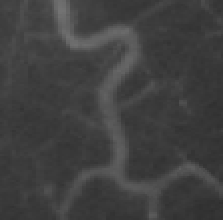
\includegraphics[width=0.24\textwidth]{images/L2S_compare/orig_4}	&
\includegraphics[width=0.24\textwidth]{images/L2S_compare/GAC_4}	&
\includegraphics[width=0.24\textwidth]{images/L2S_compare/CV_4}		&
\includegraphics[width=0.24\textwidth]{images/L2S_compare/L2S_4}	
\\
\includegraphics[width=0.24\textwidth]{images/L2S_compare/orig_5}	&
\includegraphics[width=0.24\textwidth]{images/L2S_compare/GAC_5}	&
\includegraphics[width=0.24\textwidth]{images/L2S_compare/CV_5}		&
\includegraphics[width=0.24\textwidth]{images/L2S_compare/L2S_5}	\\
(a) original image & (b) GAC & (c) Chan Vese & (d) L2S
\end{tabular}
\caption[L2S vs GAC vs Chan-Vese]{(a) A 2D image. Segmentation via (b) Geodesic active contour, (c)Chan-Vese and (d)L2S. The initial contour is plotted in green and the final contour in yellow. Intermediate steps of curve evolution are shown in cyan. Best viewed in color.}
\label{fig:l2s_compare_GAC_CV}
\end{figure*}
In Chapter ~\ref{Chapter3}, we introduced the edge based Geodesic active contour\cite{caselles_geodesic} model and region based technique due to Chan and Vese \cite{chan_vese}. Fig.~\ref{fig:l2s_compare_GAC_CV} shows the performance of L2S versus GAC and Chan-Vese's method. To maintain fairness of comparison, we have initialized the level set at the same positions for each methods (shown by the green contour). All the five images used for this demonstration are characterized by low contrast, weak edges and significant variation in region illumination levels. GAC and Chan-Vese's algorithm's performance is limited due to these artifacts. GAC is prone to error due to weak edges causing contour leakage, whereas the piecewise constant model due to Chan and Vese is unable to accomodate the intensity inhomogeneities. However, we observe that L2S exhibits significantly superior qualitative performance since it is (a) not dependent on the edge information and (b) capable of handling discontinuities by using polynomial approximation for region intensities.

\clearpage
\subsection{Comparison with other methods}
To demonstrate the efficacy of the proposed method, we perform further experiments on a dataset of 32 images. The dataset consists of a set of synthetic images with added noise and simulated intensity inhomogeneity, a set of biomedical images consisting of blood vessels using magnetic resonance angiogram (MRA), neurons and dendritic spines imaged by confocal microscope and finally, a set of ultrasound images of human blood vessels.  

To evaluate the performance of L2S, we compare our approach with three popular and widely used region based segmentation algorithms viz. Chan-Vese \cite{chan_vese}, Lankton et. al. \cite{lankton_localCV} and Li et. al.\cite{li_region_scalable}. We use the freely available CREASEG\cite{creaseg} tool to evaluate the performance. We choose the above techniques for performance evaluation since all the above models (barring Chan-Vese) were developed to perform region based segmentation with varying object brightness.

To set up the comparative evaluation procedure, we first present the segmentation results on a biomedical image dataset containing vascular structures. This is shown in Fig.~\ref{fig:l2s_compare_vessels}. Fig.~\ref{fig:l2s_compare_vessels}(a) shows the original microscopy images with the initial contour shown in yellow, followed by segmentation results due to (b) Chan-Vese in blue, (c) Lankton \textit{et al.} in red, (d) Li \textit{et al.} in cyan and finally (e) L2S (yellow). The images contains vascular structures and are characterized by  noise, non-object clutter and inhomogeneous intensity. To make a fair evaluation, the images were not preprocessed for contrast improvement or noise removal. Qualitative results suggest the efficacy of L2S in delineating vascular objects in non ideal scenarios.

\begin{figure*}[t]
\centering
\renewcommand{\tabcolsep}{0.05cm}
\begin{tabular}{@{}ccccc@{}}
\includegraphics[width=0.19\textwidth]{images/L2S_compare_region/19_orig}	&
\includegraphics[width=0.19\textwidth]{images/L2S_compare_region/19_CV}	&
\includegraphics[width=0.19\textwidth]{images/L2S_compare_region/19_Lankton}		&
\includegraphics[width=0.19\textwidth]{images/L2S_compare_region/19_Li}	&
\includegraphics[width=0.19\textwidth]{images/L2S_compare_region/19_ours}	
\\
\includegraphics[width=0.19\textwidth]{images/L2S_compare_region/22_trng_orig}	&
\includegraphics[width=0.19\textwidth]{images/L2S_compare_region/22_trng_CV}	&
\includegraphics[width=0.19\textwidth]{images/L2S_compare_region/22_trng_Lankton}		&
\includegraphics[width=0.19\textwidth]{images/L2S_compare_region/22_trng_Li}	&
\includegraphics[width=0.19\textwidth]{images/L2S_compare_region/22_trng_ours}	
\\
\includegraphics[width=0.19\textwidth]{images/L2S_compare_region/dendrites2_orig}	&
\includegraphics[width=0.19\textwidth]{images/L2S_compare_region/dendrites2_CV}	&
\includegraphics[width=0.19\textwidth]{images/L2S_compare_region/dendrites2_Lankton} &
\includegraphics[width=0.19\textwidth]{images/L2S_compare_region/dendrites2_Li}	&
\includegraphics[width=0.19\textwidth]{images/L2S_compare_region/dendrites2_ours}	
\\
\includegraphics[width=0.19\textwidth]{images/L2S_compare_region/n13_orig}	&
\includegraphics[width=0.19\textwidth]{images/L2S_compare_region/n13_CV}	&
\includegraphics[width=0.19\textwidth]{images/L2S_compare_region/n13_Lankton} &
\includegraphics[width=0.19\textwidth]{images/L2S_compare_region/n13_Li}	&
\includegraphics[width=0.19\textwidth]{images/L2S_compare_region/n13_ours}	
\\
\includegraphics[width=0.19\textwidth]{images/L2S_compare_region/neuron_clear_orig}	&
\includegraphics[width=0.19\textwidth]{images/L2S_compare_region/neuron_clear_CV}	&
\includegraphics[width=0.19\textwidth]{images/L2S_compare_region/neuron_clear_Lankton} &
\includegraphics[width=0.19\textwidth]{images/L2S_compare_region/neuron_clear_Li}	&
\includegraphics[width=0.19\textwidth]{images/L2S_compare_region/neuron_clear_ours}	
\\
\includegraphics[width=0.19\textwidth]{images/L2S_compare_region/spine2_orig}	&
\includegraphics[width=0.19\textwidth]{images/L2S_compare_region/spine2_CV}	&
\includegraphics[width=0.19\textwidth]{images/L2S_compare_region/spine2_Lankton} &
\includegraphics[width=0.19\textwidth]{images/L2S_compare_region/spine2_Li}	&
\includegraphics[width=0.19\textwidth]{images/L2S_compare_region/spine2_ours}	
\\
\includegraphics[width=0.19\textwidth]{images/L2S_compare_region/Vessel_CTA1_orig}&
\includegraphics[width=0.19\textwidth]{images/L2S_compare_region/Vessel_CTA1_CV}	&
\includegraphics[width=0.19\textwidth]{images/L2S_compare_region/Vessel_CTA1_Langton} &
\includegraphics[width=0.19\textwidth]{images/L2S_compare_region/Vessel_CTA1_Li}	&
\includegraphics[width=0.19\textwidth]{images/L2S_compare_region/Vessel_CTA1_ours}	
\\
\includegraphics[width=0.19\textwidth]{images/L2S_compare_region/vessel1_orig}	&
\includegraphics[width=0.19\textwidth]{images/L2S_compare_region/vessel1_CV}	&
\includegraphics[width=0.19\textwidth]{images/L2S_compare_region/vessel1_Lankton} &
\includegraphics[width=0.19\textwidth]{images/L2S_compare_region/vessel1_Li}	&
\includegraphics[width=0.19\textwidth]{images/L2S_compare_region/vessel1_ours}	
\\
\scriptsize(a)2D image&\scriptsize(b)Chan-Vese&\scriptsize(c)Lankton \textit{et al}\cite{lankton_localCV}&\scriptsize(d)Li \textit{et al}\cite{li_region_scalable}&\scriptsize(e)L2S
\end{tabular}
\caption[L2S on vascular images]{Qualitative comparison of L2S for vascular images.}
\label{fig:l2s_compare_vessels}
\end{figure*}
\clearpage

\begin{figure*}[t]
\centering
\renewcommand{\tabcolsep}{0.05cm}
\begin{tabular}{@{}ccccc@{}}
\includegraphics[width=0.19\textwidth]{images/L2S_compare_region/Degrade_orig}	&
\includegraphics[width=0.19\textwidth]{images/L2S_compare_region/Degrade_CV}	&
\includegraphics[width=0.19\textwidth]{images/L2S_compare_region/Degrade_Lankton}		&
\includegraphics[width=0.19\textwidth]{images/L2S_compare_region/Degrade_Li}	&
\includegraphics[width=0.19\textwidth]{images/L2S_compare_region/Degrade_ours}	
\\
\includegraphics[width=0.19\textwidth]{images/L2S_compare_region/SIM2_orig}	&
\includegraphics[width=0.19\textwidth]{images/L2S_compare_region/SIM2_CV}	&
\includegraphics[width=0.19\textwidth]{images/L2S_compare_region/SIM2_Lankton}		&
\includegraphics[width=0.19\textwidth]{images/L2S_compare_region/SIM2_Li}	&
\includegraphics[width=0.19\textwidth]{images/L2S_compare_region/SIM2_ours}	
\\
\includegraphics[width=0.19\textwidth]{images/L2S_compare_region/mushroom_orig}	&
\includegraphics[width=0.19\textwidth]{images/L2S_compare_region/mushroom_CV}	&
\includegraphics[width=0.19\textwidth]{images/L2S_compare_region/mushroom_Lankton} &
\includegraphics[width=0.19\textwidth]{images/L2S_compare_region/mushroom_Li}	&
\includegraphics[width=0.19\textwidth]{images/L2S_compare_region/mushroom_ours}	
\\
\includegraphics[width=0.19\textwidth]{images/L2S_compare_region/Airplane_orig}	&
\includegraphics[width=0.19\textwidth]{images/L2S_compare_region/Airplane_CV}	&
\includegraphics[width=0.19\textwidth]{images/L2S_compare_region/Airplane_Lankton} &
\includegraphics[width=0.19\textwidth]{images/L2S_compare_region/Airplane_Li}	&
\includegraphics[width=0.19\textwidth]{images/L2S_compare_region/Airplane_ours}	
\\
\includegraphics[width=0.19\textwidth]{images/L2S_compare_region/muscle_orig}	&
\includegraphics[width=0.19\textwidth]{images/L2S_compare_region/muscle_CV}	&
\includegraphics[width=0.19\textwidth]{images/L2S_compare_region/muscle_Lankton}		&
\includegraphics[width=0.19\textwidth]{images/L2S_compare_region/muscle_Li}	&
\includegraphics[width=0.19\textwidth]{images/L2S_compare_region/muscle_ours}	
\\
\includegraphics[width=0.19\textwidth]{images/L2S_compare_region/US3_orig}	&
\includegraphics[width=0.19\textwidth]{images/L2S_compare_region/US3_CV}	&
\includegraphics[width=0.19\textwidth]{images/L2S_compare_region/US3_Lankton} &
\includegraphics[width=0.19\textwidth]{images/L2S_compare_region/US3_Li}	&
\includegraphics[width=0.19\textwidth]{images/L2S_compare_region/US3_ours}	
\\
\includegraphics[width=0.19\textwidth]{images/L2S_compare_region/US7_orig}	&
\includegraphics[width=0.19\textwidth]{images/L2S_compare_region/US7_CV}	&
\includegraphics[width=0.19\textwidth]{images/L2S_compare_region/US7_Lankton} &
\includegraphics[width=0.19\textwidth]{images/L2S_compare_region/US7_Li}	&
\includegraphics[width=0.19\textwidth]{images/L2S_compare_region/US7_ours}	
\\
\includegraphics[width=0.19\textwidth]{images/L2S_compare_region/yeast_orig}	&
\includegraphics[width=0.19\textwidth]{images/L2S_compare_region/yeast_CV}	&
\includegraphics[width=0.19\textwidth]{images/L2S_compare_region/yeast_Lankton} &
\includegraphics[width=0.19\textwidth]{images/L2S_compare_region/yeast_Li}	&
\includegraphics[width=0.19\textwidth]{images/L2S_compare_region/yeast_ours}\\
\scriptsize(a)2D image&\scriptsize(b)Chan-Vese&\scriptsize(c)Lankton \textit{et al}\cite{lankton_localCV}&\scriptsize(d)Li \textit{et al}\cite{li_region_scalable}&\scriptsize(e)L2S
\end{tabular}
\caption[L2S on vascular images]{Qualitative comparison of L2S for non vascular images.}
\label{fig:l2s_compare_nonvessel}
\end{figure*}
\clearpage
We had mentioned earlier that one of our goals is to develop a segmentation procedure which is reasonably widely applicable. In this chapter we do not assume any structural prior for the objects to be segmented. Although prior information may achieve better results, the algorithm loses its general applicability. In the following chapter we will present a more problem specific solution to neuron segmentation. Since L2S is a general purpose segmentation algorithm, we also present qualitative results on non-vascular structures. However, almost all these images are characterized by inhomogeneous contrast, which is the major issue we try to address in this chapter. 

Segmentation results on a few representative images are  shown in Fig.~\ref{fig:l2s_compare_nonvessel}. This set of non vessel images belong to different categories. The first two images are simulated to contain a varying contrast and additive noise. We also include MRI images of human leg muscles, natural images from the Berkeley segmentation database\cite{BerkeleySegDatabase}, noisy ultrasound images of human arteries and finally microscopy images of yeast cells. As before, L2S results are shown in yellow and qualitative comparison suggest robustness of the method.

\subsection{Quantitative performance evaluation}
The Dice coefficient \cite{bernard_splinedCV} is used to quantify the results of segmentation. The Dice index $\mathcal{D}\in [0,1]$ between two regions $R_1$ and $R_2$ is given by 
\bea
\mathcal{D}(R_1,R_2)=2\dfrac{|R_1\cap R_2|}{|R_1|+|R_2|}
\label{eq:Dice}
\eea
Here $R_2$ is a binary image that denotes ground truth segmentation, and $R_1$ is the result obtained experimentally. A Dice index of 1 indicates perfect segmentation. The quantitative performance is shown in Fig.~\ref{fig:L2S_Dice}. 
\begin{figure}[t]
\centering
\includegraphics[width=1\textwidth]{images/L2S_Dice}
\caption[Quantitative comparison of L2S]{Dice index for the different algorithms are plotted in this bar chart. L2S results are shown by the yellow bar. Best viewed in color.}	
\label{fig:L2S_Dice}
\end{figure}
We observe that over this entire dataset, L2S yields an average Dice score of $0.9$, compared to $0.62,0.57$ and $0.7$ for the methods described in \cite{chan_vese},\cite{lankton_localCV} and \cite{li_region_scalable} respectively. 

\subsection{Computational comparison}
\begin{figure}[b]
\centering
\includegraphics[width=0.8\textwidth]{images/L2S_time}
\caption[Computational comparison for L2S]{The CPU running times (sec) for the different algorithms are plotted in this bar chart. L2S results are shown by the yellow bar. Best viewed in color.}	
\label{fig:L2S_comput}
\end{figure}
Our algorithm is implemented in Matlab and all experiments are performed on an Intel Pentium processor with 16 GB memory. The convergence times (in seconds) for the four algorithms are presented in Fig.~\ref{fig:L2S_comput}. Computationally, our method outperforms  \cite{lankton_localCV} and \cite{li_region_scalable} on average. It may be noted that the apparent low convergence time of \cite{chan_vese} often is a result of  convergence at local minima, which do not necessarily correspond to correct object boundaries.

\subsection{Discussion}
A novel framework for segmentation in presence of significant intra-region illumination variation is presented. Qualitative and quantitative results and comparison with the state of the art techniques suggest robustness of our approach. Here we have focused on bi-level segmentation, although extension to a multi-level framework appears straightforward. Also, our formulation allows easy incorporation of \textit{a priory} shape information, which may enhance performance in select cases. Salient highlights of L2S are presented below:
\begin{itemize}
\item L2S uses geometric active contours for segmentation. Therefore, it can adapt to the topological variations in objects via automatic merging and splitting.
\item L2S is robust against inhomogeneous intensity levels caused by non uniform signal attenuation or external bias fields, which occurs in many biological imaging applications. 
\item L2S is a region based method and its performance is robust against noise and weak edges.
\item L2S is computationally efficient and numerically stable.
\end{itemize}

However, like most level set methods, L2S is somewhat biased towards contour initialization. 
Also, although Legendre polynomials for region intensity approximation provides an elegant solution, it is difficult to comment on the optimality of this choice of basis. Effectiveness of other polynomials such as splines or wavelets \cite{achuthan2010wavelet} needs further investigation. In select cases, it may also be possible to learn a compact set of bases for representation. To address this issue, we focus our attention to an application where a set of training examples of the object is available. We show that in such applications, the region approximating polynomials may be learned efficiently, instead of pre specifying them. This leads to the next topic of discussion, \textit{Dictionary Learning Level Sets}.

\section{Dictionary Learning Level Sets (DL2S)}

The primary motivation for DL2S is similar to that of L2S-- performing segmentation in presence of intensity inhomogeneity. In L2S\cite{mukherjee_L2S}, we generalized the Chan-Vese model by approximating the foreground and background regions as a piecewise polynomial function  computed via linear combination of a few Legendre basis functions. This can be viewed from the perspective of low dimensional approximation of a signal.  While Chan-Vese's method is a form of extreme dimensionality reduction (due to the piecewise constant assumption), L2S achieves a balance between reduction of dimensionality and accurate intensity modeling. 

Despite its merits, L2S suffers from certain issues. First, the segmentation quality relies heavily on the number of chosen basis functions. Second,  L2S suffers from scalability issues since the pre-specified bases cannot represent any arbitrary intensity variation. As it turns out, recent research in the field of sparse modeling and dictionary learning\cite{sparse_face,dl_algo,elad_denoising,dl_restoration,elad_ksvd} have shown that for a given set of training data, one can obtain an optimal set of basis elements (atoms) to represent a signal. This is the main highlight of DL2S --\emph{instead of explicitly specifying the set of basis elements, we estimate an optimal set of bases from the set of training images using dictionary learning}.
\begin{figure}[t]
\centering
	\renewcommand{\tabcolsep}{0.05cm}
	\renewcommand{\arraystretch}{0.05}
	\begin{tabular}{@{}ccc@{}}
		\includegraphics[width=.3\linewidth]{./images/DL2S/compare/vessINVIVO2_orig} &
		\includegraphics[width=.3\linewidth]{./images/DL2S/compare/vessINVIVO2_CV} &
		\includegraphics[width=.3\linewidth]{./images/DL2S/compare/vessINVIVO2_DL} 
		\\
		\includegraphics[width=.3\linewidth]{./images/DL2S/compare/imCyl2_orig} &		
		\includegraphics[width=.3\linewidth]{./images/DL2S/compare/imCyl2_CV} &
		\includegraphics[width=.3\linewidth]{./images/DL2S/compare/imCyl2_DL}
		\\ 
		\includegraphics[width=.3\linewidth]{./images/DL2S/compare/vessFIRvol15_orig}&
 		\includegraphics[width=.3\linewidth]{./images/DL2S/compare/vessFIRvol15_CV} &
		\includegraphics[width=.3\linewidth]{./images/DL2S/compare/vessFIRvol15_DL} 
	\end{tabular}
\caption[Chan-Vese vs DL2S]{Segmentation results of Chan-Vese\cite{chan_vese} (white) and DL2S (yellow) on three C-mode ultrasound images captured with a portable scanner.}
\label{fig:viz_comp}
\end{figure}
To demonstrate our technique, we choose an important segmentation problem for ultrasound imaging. Blood vessels are imaged in C-mode using a portable, low cost, battery operated ultrasound device. Our objective is to segment the vessel boundary to assist medical practitioners for performing phlebotomy application such as intravenous needle placement (see Fig.~\ref{fig:viz_comp}). Images captured using these portable devices suffer from low contrast, noise and speckle in addition to non-linear illumination of the objects which makes segmentation challenging. 
\subsection{Methodology}
A generalized version of Chan-Vese's model can be  formulated as follows:
\bea
\mathcal{E}(\phi,A,B)&=\displaystyle
\int_{\Omega}|f(\textbf{x})-\sum_{i=0}^{k}a_id_i(\textbf{x})|^2 m_1(\textbf{x}) d\textbf{x}   +\int_{\Omega}|f(\textbf{x})-\sum_{i=0}^{k}b_id_i(\textbf{x})|^2 m_2(\textbf{x}) d\textbf{x}  \nn \\
						  &+ \displaystyle \nu \int_{\Omega} |\nabla\heav(\phi)|
						   d\textbf{x} + \lambda \left(||A||_2^2+||B||_2^2\right)
\label{eq:dl_ls_mat}
\eea
Here $\mathbb{D}_k(\textbf{x})=\left[d_1(\textbf{x}),\ldots,d_k(\textbf{x})\right]^T$ is a dictionary which will be discussed in detail shortly. $d_0(\textbf{x})=\textbf{1}$. $d_1,\ldots,d_k$ are dictionary elements or atoms which are used to model the non-linearity in the intra-region intensities of the images. The third term in (\ref{eq:dl_ls_mat}) introduces smoothness in the solution, which is controlled using the parameter $\nu$. $A=\left[a_0,\ldots,a_k\right]^T,B=\left[b_0,\ldots,b_k\right]^T$ are $(k+1)$ dimension real valued coefficient vectors. The parameter $\lambda$ reduces over-fitting, by constraining the $\ell_2$ norm of the coefficient vectors.

With $k=0$, (\ref{eq:dl_ls_mat}) reduces to the piecewise constant model in (\ref{eq:chan_vese}). In other words, (\ref{eq:dl_ls_mat}) generalizes the traditional Chan-Vese technique by introducing capability to handle heterogeneous image regions. Here $d_1,\ldots,d_k$ can be interpreted as \textit{detail functions} to model the intensity variation in conjunction to the constant illumination term $d_0$. As earlier, (\ref{eq:dl_ls_mat}) can be optimized with respect to $\phi,A\; \text{and}\; B$ using alternating minimization.  

Naturally, a question arises-- how to select  $d_1(\textbf{x}),\ldots,d_k(\textbf{x})$? It was shown in \cite{mukherjee_L2S} that high quality segmentation results can be obtained by using a few Legendre basis functions. However, we hypothesize that if a dataset of example images is available, we can enhance the segmentation performance by learning an optimal set of basis functions (dictionary elements) for region intensity approximation instead of using a predefined set of basis.
For the application described in this paper, we are concerned with sets of ultrasound images, imaged using similar type of devices. The multi-depth images are captured at the same scale, and are preregistered. As a result, we have the provision to learn these functions $d_i(\textbf{x})$ directly from the dataset, rather than relying on \textit{ad hoc} procedures for selecting the same.

\subsection{Intensity modeling with dictionary learning}
Sparse coding techniques have gained popularity recently. Such algorithms have been used for a multitude of applications ranging from image denoising, inpainting, restoration, classification, retrieval etc \cite{elad_denoising,dl_algo,sparse_face,dl_restoration}. Given a set of training data, the goal of dictionary learning is to compute a set of basis elements, also called  \textit{atoms}, such that each training data can be represented as a linear combination of only a few of these atoms. The key idea is to utilize the underlying sparsity of the training data, while minimizing the reconstruction error. 
Mathematically, if $\mathbb{F}=\left[f_1,\ldots,f_N\right]$ denotes the set of $N$ discretized, vectorized and mean subtracted training images, we can use dictionary learning technique to compute the dictionary $\mathbb{D}_k=\left[d_1,\ldots,d_k\right]^T$ mentioned in (\ref{eq:dl_ls_mat}) by solving the following optimization problem
\bea
\mathbb{D}_k=\text{arg}\min_{\mathbb{D},y_i} \sum_{i=1}^{N}||f_i-\mathbb{D}^Ty_i||_2^2 \nn \\
 \text{such that}\; ||y_i||_0 \leq \theta, \;\;\; \forall i=1,...,N.
 \label{eq:DL}
\eea
where $y_i$ is a coefficient vector corresponding to the $i^{th}$ training image and $\theta$ is a scalar which dictates the level of sparsity. There are a number of methods in the literature that use some approximation to solve the hard optimization problem (\ref{eq:DL}). For example, k-SVD \cite{elad_ksvd} combines a greedy methodology using orthogonal matching pursuit algorithm to provide a fast solution to this problem. Dictionary learning exploits sparsity in the data (\ref{eq:DL}) by constraining $\ell_0$ norm of the coefficients.

\subsection{DL2S curve evolution}
Let us denote $\mathbb{\hat{D}}_k=[d_0(\textbf{x})^T\; \mathbb{D}_k(\textbf{x})]^T$. We first try to minimize (\ref{eq:dl_ls_mat}) with respect to $A$ and $B$, by taking derivatives and setting the result to zero. A closed form solution  is obtained as follows:
\bea
\hat{A} =& \left[K+ \lambda \mathbb{I}\right]^{-1}\displaystyle\int_{\Omega} \mathbb{\hat{D}}(\textbf{x})f(\textbf{x})m_1(\textbf{x})d\textbf{x}  \\
\hat{B} =& \left[L+ \lambda \mathbb{I}\right]^{-1}\displaystyle\int_{\Omega}  \mathbb{\hat{D}}(\textbf{x})f(\textbf{x})m_2(\textbf{x})d\textbf{x}
\label{eq:coef_sol}
\eea
where $\left[. \right]$ denotes a matrix. $\left[K \right]$ and $\left[L \right]$ are $k\times k$ Gramian matrices \cite{gramian}, in which $(i,j)^{th}$ entries are obtained as
\bea
\left[K\right]_{i,j}= m_1(\textbf{x})\left<d_i,d_j\right> \, \text{and} \,
\left[L\right]_{i,j}= m_2(\textbf{x})\left<d_i,d_j\right>
\eea
$0\leq i,j \leq k$ and $\left<,\right>$ denotes the Euclidean inner product operator. With the updated coefficient vectors, we can now minimize (\ref{eq:dl_ls_mat}) with respect to $\phi$ using variational calculus. We obtain the following partial differential equation using gradient descent technique for minimization.
\bea
\frac{\partial \phi}{\partial t}=\left[-|f(\textbf{x})-\hat{A}^T\mathbb{\hat{D}}_k(\textbf{x})|^2 
						   +|f(\textbf{x})-\hat{B}^T\mathbb{\hat{D}}_k(\textbf{x})|^2 \right]\dirac(\phi) 
						  +  \nu \dirac(\phi)\text{div}\left(\frac{\nabla\phi}{|\nabla\phi|}\right) \nn \\
\label{eq:Dl2S_final_PDE}						  
\eea
We initialize $\phi|_{t=0}=\phi_0$ and $\dfrac{\dirac(\phi)}{|\nabla \phi|}\dfrac{\partial\phi}{\partial \hat{n}}=0$ at the domain boundary. The gradient flow of DL2S is computed iteratively by discretizing (\ref{eq:Dl2S_final_PDE}) using a finite difference scheme.
\begin{figure}[t]
\centering
	\renewcommand{\tabcolsep}{0.05cm}
	\begin{tabular}{@{}cccc@{}}
		\includegraphics[width=.24\linewidth]{./images/DL2S/evolution/cylDPSS_DLevol570} &
		\includegraphics[width=.24\linewidth]{./images/DL2S/evolution/cylDPSS_DLevol5710} &
		\includegraphics[width=.24\linewidth]{./images/DL2S/evolution/cylDPSS_DLevol5720} &
		\includegraphics[width=.24\linewidth]{./images/DL2S/evolution/cylDPSS_DLevol57221} 
		\\
		\scriptsize(a) & \scriptsize (b)&\scriptsize(c)&\scriptsize(d)
	\end{tabular}
%} 
\caption[DL2S curve evolution]{Evolution steps shown for our algorithm (a) initialization, (b) iteration=20, (c) iteration=60, (d) final contour.}
\vspace{-0.5cm}
\label{fig:DL2S_curve_evol}
\end{figure}
Fig.~\ref{fig:DL2S_curve_evol} shows different steps of the curve evolution. Fig.~\ref{fig:DL2S_curve_evol}(a) shows the initialization Fig.~\ref{fig:DL2S_curve_evol}(b) and (c) shows two intermediate steps and Fig.~\ref{fig:DL2S_curve_evol}(d) shows the finally evolved curve.

\subsection{Analysis of DL2S}
\begin{figure}[th]
\centering
\renewcommand{\tabcolsep}{0.05cm}
	\begin{tabular}{@{} c@{}}
		\includegraphics[width=.9\linewidth]{./images/DL2S/dataset1_dict} 
	\end{tabular}
\caption[DL2S dictionary]{Eight dictionary atoms learned from the mean subtracted images for a phantom image category.}
\label{fig:DLbasis}
\end{figure}
The Chan-Vese method performs segmentation by approximating an image $f(\textbf{x})$ by a piecewise constant image $g(\textbf{x})$. To make the model more flexible, we  add higher order terms which can capture the intensity variations in the regions. Going by the intuition of Chan and Vese, it is fair to approximate the mean image of a dataset as a piecewise constant image.  

Assuming a mean image which is approximately piecewise constant, the dictionary atoms learned from the mean subtracted dataset can be utilized to provide the non-linear variation necessary to model the intensity inhomogeneity. The energy functional in  (\ref{eq:dl_ls_mat}) essentially incorporates this idea in a mathematical framework. One can also think of the dictionary atoms as incorporating higher order details, learned to suit our dataset. The dictionary atoms computed for a particular ultrasound image dataset is shown in Fig.~\ref{fig:DLbasis}. The dictionary atoms aid in retaining the more significant image properties  and compactly represent the dataset. 

DL2S is applicable where a set of pre-registered training data is available, for example multi-depth ultrasound images of blood vessels, in temporal image sequences of biomedical objects such as carotid artery, heart videos. In applications involving a temporal image sequence, the first few frames of the can be treated as the training data to learn the dictionary, which can be exploited to segment the subsequent frames.    

\subsection{Experimental Results}
We use five different sets of images to evaluate the performance of our algorithm. Out of them, three datasets contain images of medical phantoms which mimic human veins. These phantoms are generally used by medical practitioners for device calibration. The remaining two datasets consists of human vein images, captured \textit{in vivo}. Each dataset contains approximately 18 to 60 images, captured in C-mode using a portable, battery operated ultrasound scanner. The different images in a given set correspond to the image of a vein at various depths. Note that each dataset consists of registered blood vessel images. The vessel orientation and scale are also consistent. A separate dictionary is computed using the mean subtracted images for each of the datasets. 
\begin{figure}[b]
\centering
\renewcommand{\tabcolsep}{0.05cm}
\begin{tabular}{@{}cccc@{}}
			\includegraphics[width=.24\linewidth]{./images/DL2S/Initialization/init_ell} &
			\includegraphics[width=.24\linewidth]{./images/DL2S/Initialization/vessINVIVO02_CV_ell} &
			\includegraphics[width=.24\linewidth]{./images/DL2S/Initialization/vessINVIVO02_L2S_p2_ell} &
			\includegraphics[width=.24\linewidth]{./images/DL2S/Initialization/vessINVIVO02_DL_ell} 
			\\ 
			\includegraphics[width=.24\linewidth]{./images/DL2S/Initialization/init_mb} &
			\includegraphics[width=.24\linewidth]{./images/DL2S/Initialization/vessINVIVO02_CV_mb} &
			\includegraphics[width=.24\linewidth]{./images/DL2S/Initialization/vessINVIVO02_L2S_p2_mb} &
			\includegraphics[width=.24\linewidth]{./images/DL2S/Initialization/vessINVIVO02_DL_mb} 
			\\
		    \scriptsize(a) & \scriptsize (b) &\scriptsize (c) & \scriptsize (d)
\end{tabular}
\caption[DL2S initialization robustness]{Comparison of segmentation results using manual and automatic initialization methods. (a) initialized contour (b) segmentation results of Chan-Vese (white), (c) segmentation via L2S (black) and (d) segmentation via DL2S model (yellow)}
\label{fig:init_compare}
\end{figure}

\textbf{Dependency on contour initialization}: We show the performance of our algorithm using both manual and automatic initialization methods. The segmentation results with manual and automatic initialization for Chan-Vese\cite{chan_vese}, L2S \cite{mukherjee_L2S} and DL2S are shown in Fig.~ \ref{fig:init_compare} for the same image. We observe that the segmentation performance of L2S drops significantly for automatic initialization, which is also true for Chan-Vese method. In comparison DL2S has similar segmentation results for both initialization technique. Quantitative evaluation of performance based on initialization is provided in Table I.
\begin{figure}[t]
\centering
	\renewcommand{\tabcolsep}{0.05cm}
	\begin{tabular}{@{}cccc@{}}
		%\raisebox{0.2in}{(a)} &
		\includegraphics[width=.23\linewidth]{./images/DL2S/compare/cylNORM57_orig} &
		\includegraphics[width=.23\linewidth]{./images/DL2S/compare/cylNORM57_CV} &
		\includegraphics[width=.23\linewidth]{./images/DL2S/compare/cylNORM57_L2S_p2_c} &
		\includegraphics[width=.23\linewidth]{./images/DL2S/compare/cylNORM57_DL} 
		\\
		\includegraphics[width=.23\linewidth]{./images/DL2S/compare/cylNORM59_orig} &
		\includegraphics[width=.23\linewidth]{./images/DL2S/compare/cylNORM59_CV} &
		\includegraphics[width=.23\linewidth]{./images/DL2S/compare/cylNORM59_L2S_p2_c} &
		\includegraphics[width=.23\linewidth]{./images/DL2S/compare/cylNORM59_DL} 
		\\
		\includegraphics[width=.23\linewidth]{./images/DL2S/compare/cylDPSS58_orig} &
		\includegraphics[width=.23\linewidth]{./images/DL2S/compare/cylDPSS58_CV} &
		\includegraphics[width=.23\linewidth]{./images/DL2S/compare/cylDPSS58_L2S_p2_c}&				
		\includegraphics[width=.23\linewidth]{./images/DL2S/compare/cylDPSS58_DL}
		\\
		\includegraphics[width=.23\linewidth]{./images/DL2S/compare/vessFIRvol10_orig} &
		\includegraphics[width=.23\linewidth]{./images/DL2S/compare/vessFIRvol10_CV} &
		\includegraphics[width=.23\linewidth]{./images/DL2S/compare/vessFIRvol10_L2S_p2_c} &
		\includegraphics[width=.23\linewidth]{./images/DL2S/compare/vessFIRvol10_DL} 
		\\		
		\includegraphics[width=.23\linewidth]{./images/DL2S/compare/vessFIRvol18_orig} &
		\includegraphics[width=.23\linewidth]{./images/DL2S/compare/vessFIRvol18_CV} &		
		\includegraphics[width=.23\linewidth]{./images/DL2S/compare/vessFIRvol18_L2S_p2_c} &		
		\includegraphics[width=.23\linewidth]{./images/DL2S/compare/vessFIRvol18_DL} 
		\\		
		\includegraphics[width=.23\linewidth]{./images/DL2S/compare/vessINVIVO15_orig} &
		\includegraphics[width=.23\linewidth]{./images/DL2S/compare/vessINVIVO15_CV} &		
		\includegraphics[width=.23\linewidth]{./images/DL2S/compare/vessINVIVO15_L2S_p2_c} &		
		\includegraphics[width=.23\linewidth]{./images/DL2S/compare/vessINVIVO15_DL} 
		\\		
		\includegraphics[width=.23\linewidth]{./images/DL2S/compare/vessINVIVO17_orig} &
		\includegraphics[width=.23\linewidth]{./images/DL2S/compare/vessINVIVO17_CV}   &
		\includegraphics[width=.23\linewidth]{./images/DL2S/compare/vessINVIVO17_L2S_p2_c} & 
		\includegraphics[width=.23\linewidth]{./images/DL2S/compare/vessINVIVO17_DL} 
	\end{tabular}
\caption[Qualitative comparison of DL2S]{Segmentation comparison of DL2S with Chan-Vese and L2S is shown here. The original C-mode ultrasound images captured with a portable scanner are shown in the first column. Segmentation results of Chan-Vese (white), L2S (black) and DL2S model (yellow) on these images are shown in columns 2, 3 and 4 respectively.}
\label{fig:seg_comp}
\end{figure}

\textbf{Dependency on dictionary size}: We perform sensitivity analysis experiment to study the performance of the segmentation algorithm  with changing dictionary size. The Dice coefficient are plotted (along Y-axis) for L2S \cite{mukherjee_L2S} (Fig.~\ref{fig:quant_compPolydeg} (a)) ans DL2S (Fig.~\ref{fig:quant_compPolydeg} (b)) to show the performance with changing basis / dictionary size (along X-axis) for 7 randomly chosen images. In comparison to L2S, where performance decreases with increasing number of basis functions, DL2S exhibits a more stable performance. Based on experiment evaluation, we fix the number of dictionary elements $k=8$ which is at most 50\% of the size of the smallest dataset. We choose sparsity inducing parameter $\theta=3$ such that about 30\% or less number of atoms can be used for representing the training images.
\begin{figure}[t]
\centering
\renewcommand{\tabcolsep}{0.05cm}
\begin{tabular}{cc}
	\includegraphics[width=.48\linewidth]{./images/DL2S/legnum_comp}  &
	\includegraphics[width=.48\linewidth]{./images/DL2S/dictnum_comp} 
	\\
	\scriptsize(a) & \scriptsize(b)
\end{tabular}
\caption[DL2S comparison of basis elements]{(a) Dice coefficient for L2S with changing number of basis functions, (b) Dice index for the same images plotted for DL2S with changing size of dictionary}
\label{fig:quant_compPolydeg}
\end{figure}

\begin{table}[b]
	\setlength{\tabcolsep}{2pt}
	\begin{center}
\caption[DL2S quantitative comparison] {\\Quantitative comparison of the three methods} \label{tab:quatntcomp_tab}
%\resizebox{9.3cm}{!}
\begin{adjustbox}{width=1\linewidth}
{
\begin{tabular}{c|cc|cc|cc}
\hline
 \multicolumn{1}{c}{} & \multicolumn{2}{c}{\textit{DL2S}} & \multicolumn{2}{c}{\textit{Chan-Vese} \cite{chan_vese}} & \multicolumn{2}{c}{\textit{L2S} \cite{mukherjee_L2S}}\\
\hline
	\multicolumn{1}{c}{} & \underbar{\textit{Manual}} & \underbar{\textit{Auto}} & \underbar{\textit{Manual}} & \underbar{\textit{Auto}} & \underbar{\textit{Manual}} & \underbar{\textit{Auto}}\\
	%\cline{2-7}
	\multicolumn{1}{c}{} &\bf{0.93$\pm$0.02}& 0.92$\pm$0.04 & 0.91$\pm$ 0.07 & 0.86$\pm$0.11 & 0.89$\pm$0.09 & 0.55$\pm$0.17\\
	%\cline{1-7}
	\multicolumn{1}{c}{} & \bf{0.90$\pm$0.04}& \bf{0.90$\pm$0.07} & 0.88$\pm$ 0.05 & 0.88$\pm$0.12 &  \bf{0.90$\pm$0.06} & 0.88$\pm$0.12\\
	%\cline{1-7
	\multicolumn{1}{c}{} & 0.85$\pm$0.08&\bf{0.86$\pm$0.08} & 0.80$\pm$ 0.08 & 0.85$\pm$0.11 &  0.85$\pm$0.12 & 0.84$\pm$0.09\\
	%\cline{1-7}
	\multicolumn{1}{c}{} & 0.80$\pm$0.10& \bf{0.83$\pm$0.06} & 0.69$\pm$ 0.21 & 0.73$\pm$0.12 & 0.70$\pm$0.19 & 0.60$\pm$0.14\\
	%\cline{1-7}
	\multicolumn{1}{c}{} & \bf{0.76$\pm$0.16}& \bf{0.76$\pm$0.10} & 0.75$\pm$ 0.14 & 0.72$\pm$0.11 & 0.72$\pm$0.16 & 0.62$\pm$0.13\\
\hline
\end{tabular}		
}
\end{adjustbox}
\end{center}
\vspace{-0.5cm}
\end{table}
\textbf{Quantitative comparison of segmentation}: Fig.~\ref{fig:seg_comp} shows the segmentation performance of Chan-Vese (white) \cite{chan_vese}), L2S (black)\cite{mukherjee_L2S}  and DL2S (yellow) 
Fig.~\ref{fig:seg_comp} shows that DL2S is able to capture the blood vessels more appropriately in presence of severe contrast and intensity inhomogeneity. A quantitative comparison for five datasets as shown in Table~\ref{tab:quatntcomp_tab}.
The Dice index is evaluated for the three algorithms. Here $s_g$ denotes the ground truth segmentation and $s_t$ is the segmentation result for DL2S, Chan-Vese or L2S. It is observed that for each dataset, DL2S demonstrates significantly better performance than L2S or CV. Dl2S achieves  highest improvement in performance of above 65\% in one dataset and 42\% in an in-vivo dataset. On average, we observe increase in segmentation accuracy by more thab 12\% for the all the datasets. 

The mean Dice coefficient for each of the dataset is provided in the table. Results obtained using DL2S remain significantly consistent in compariosn to L2S ans Chan-vese, for both manual and automatic initialization methods and for all the five different datasets.  

\subsection{Discussion}
We have proposed a novel segmentation method which combines the idea of dictionary learning and region based variational segmentation algorithm in presence of significant clutter and heterogeneous intensity. Furthermore, DL2S outperforms the state of the art in terms of contour initialization and demonstrates accurate segmentation in cluttered images without the use of explicit shape prior. The results presented here show significant improvement in segmentation accuracy using basis functions that are computed from the data in comparison to using a fixed number of basis functions.

 
%\input{Chapters/Chapter5} 
%\input{Chapters/Chapter6} 
%\input{Chapters/Chapter7} 

%----------------------------------------------------------------------------------------
%	THESIS CONTENT - APPENDICES
%----------------------------------------------------------------------------------------

\addtocontents{toc}{\vspace{2em}} % Add a gap in the Contents, for aesthetics

\appendix % Cue to tell LaTeX that the following 'chapters' are Appendices

% Include the appendices of the thesis as separate files from the Appendices folder
% Uncomment the lines as you write the Appendices

%% Appendix A

\chapter{Appendix Title Here} % Main appendix title

\label{AppendixA} % For referencing this appendix elsewhere, use \ref{AppendixA}

\lhead{Appendix A. \emph{Appendix Title Here}} % This is for the header on each page - perhaps a shortened title

Write your Appendix content here.
%\input{Appendices/AppendixB}
%\input{Appendices/AppendixC}

\addtocontents{toc}{\vspace{2em}} % Add a gap in the Contents, for aesthetics

\backmatter

%----------------------------------------------------------------------------------------
%	BIBLIOGRAPHY
%----------------------------------------------------------------------------------------

\label{Bibliography}

%\lhead{\emph{Bibliography}} % Change the page header to say "Bibliography"

%%\bibliographystyle{unsrtnat} % Use the "unsrtnat" BibTeX style for formatting the Bibliography
\bibliographystyle{IEEEtran}
\bibliography{Bibliography} % The references (bibliography) information are stored in the file named "Bibliography.bib"

\end{document}  